% IEEEtran initializes Times before fontspec; give that initialization T1 fonts.
\RequirePackage[T1]{fontenc}
\ifdefined\ECNConferenceVersion
\documentclass[10pt,conference]{IEEEtran}
\else
\documentclass[11pt,journal,onecolumn]{IEEEtran}
\fi
\usepackage{iftex}
\ifPDFTeX
\usepackage[T1]{fontenc}
\usepackage{lmodern}
\else
\usepackage{fontspec}
\setmainfont{lmroman10-regular.otf}[BoldFont=lmroman10-bold.otf,ItalicFont=lmroman10-italic.otf,BoldItalicFont=lmroman10-bolditalic.otf,SmallCapsFont=lmromancaps10-regular.otf]
\fi
\usepackage{amsmath,amssymb,booktabs,graphicx,array}
\usepackage{microtype}
\usepackage{hyperref}
\usepackage{cite}
\usepackage{etoolbox}
\usepackage{multirow}
\setcounter{tocdepth}{2}
\IfFileExists{figures/fig1_lift_heatmap.png}{\def\HistoricalFigureRoot{figures}}{\IfFileExists{ECNBENCH-RELEASE/06_figures/fig1_lift_heatmap.png}{\def\HistoricalFigureRoot{ECNBENCH-RELEASE/06_figures}}{\def\HistoricalFigureRoot{../06_figures}}}
\appto\ttfamily{\hyphenchar\font=45}
\setlength{\emergencystretch}{3em}
\renewcommand{\topfraction}{0.9}
\renewcommand{\textfraction}{0.08}
\hypersetup{colorlinks=true,linkcolor=blue,citecolor=blue,urlcolor=blue,
pdfauthor={Minh Hien NGUYEN},pdftitle={ECN-BENCH: Design, Systems Engineering, and a Forensic Audit of Multi-Agent Forecasting}}
\newcommand{\AuditRows}{Llama-3.1-8B & 12 & 12 & 0 \\
Mistral-7B & 60 & 19 & 1 \\
Qwen2.5-7B & 60 & 0 & 0 \\}

\newcommand{\ForecastRows}{Llama-3.1-8B & 0.675 & 0.500 & 0.545 & 0.613 \\
Mistral-7B & 0.850 & 0.650 & 0.378 & 0.441 \\
Qwen2.5-7B & 0.850 & 0.550 & 0.348 & 0.520 \\
Qwen2.5-14B & 0.900 & 0.800 & 0.289 & 0.432 \\}

\newcommand{\SensitivityRows}{Evaluator A, averaged vector & 20 & $ +0.112 [+0.030, +0.192] $ \\
Evaluator A, mean read score & 20 & $ +0.114 [+0.031, +0.197] $ \\
Evaluator C, single read & 20 & $ +0.081 [-0.003, +0.170] $ \\
A, excluding input/gap events & 16 & $ +0.116 [+0.026, +0.206] $ \\
A, US election grouped & 20 & $ +0.112 [+0.034, +0.195] $ \\
A, excluding US election & 14 & $ +0.117 [+0.013, +0.218] $ \\}

\newcommand{\NoiseRows}{Llama-3.1-8B & 4 & 3/90 & 0.330 \\
Mistral-7B & 4 & 0/90 & 0.375 \\
Qwen2.5-7B & 4 & 4/90 & 0.280 \\
Qwen2.5-14B & 3 & 3/90 & 0.208 \\}

\newcommand{\CotRows}{Llama-3.1-8B & Yes & 0.778 & $ -0.181 [-0.366, -0.020] $ \\
Qwen2.5-7B & Yes & 0.790 & $ -0.030 [-0.134, +0.082] $ \\
Mistral-8B & No & 0.912 & $ -0.170 [-0.371, +0.010] $ \\
Qwen3-14B & No & 0.858 & $ -0.008 [-0.114, +0.092] $ \\}

\newcommand{\TruncationRows}{2k & 7/59 & 5/59 \\
5k & 4/60 & 2/60 \\
8k & 0/60 & 4/60 \\
full & 1/60 & 0/60 \\}

\newcommand{\PooledBrier}{+0.112 [+0.030, +0.192]}

\newcommand{\EvaluatorCBrier}{+0.081 [-0.003, +0.170]}

\newcommand{\MatchedCotBrier}{-0.106 [-0.226, +0.008]}

\newcommand{\PooledAccuracy}{81.9}

\newcommand{\CotAccuracy}{83.4}

\title{ECN-BENCH: Design, Systems Engineering,\\and a Forensic Audit of Multi-Agent Forecasting\\[0.3em]\large Full Technical Report}
\author{Minh Hien NGUYEN%
\thanks{Primary and corresponding author. Student no.~21618468; L2 EEA
(Bi-disciplinaire), minor in Mechanics, Facult\'e des Sciences et Ing\'enierie,
Sorbonne Universit\'e. Email: \texttt{nguyen.minh\_hien@etu.sorbonne-universite.fr}.
Scientific analysis revised September 6, 2026; authorship and repository metadata updated
September 10, 2026. This revision adds no simulation runs or evaluator calls.}}
\begin{document}
\maketitle

\begin{abstract}
An LLM that converts a multi-agent transcript into a probability distribution
is part of the forecasting system, rather than a neutral scoring function.
We study this measurement boundary through a retrospective audit of ECN-BENCH,
a social-simulation testbed with four campaigns carrying 30 event identifiers each.
On 132 simulated units with identical stored evidence, questions and options,
near-uniform forecasts occur in 31 readings by the original extractor and one
reading by a replacement. Repeated readings by the replacement also vary:
the mean within-unit Brier range is 0.208--0.375 across campaigns.
These observations establish sensitivity to the deployed extraction configuration;
they do not identify a uniquely correct reading of the swarm.
A source audit documents schema bypass and silent failure handling, but changing
the evaluator also changes other configuration details. An existing truncation
and enforcement experiment on a proxy model does not establish either factor
as the cause of the original near-uniform outputs.
Exploratory forecasting results are evaluated separately. On 20 events resolving
after the campaign models' release dates, the Brier contrast between the two
simulation conditions is $\PooledBrier$ under averaged replacement-evaluator
readings and $\EvaluatorCBrier$ under another evaluator, with event-cluster
95\% bootstrap intervals. The latter includes zero. This subset is not protected
against evaluator knowledge leakage; some injections target the wrong event,
and the null payloads are not length-matched. An existing single-agent baseline
does not establish a simulation advantage. The contribution is an auditable
case study of extraction sensitivity, with explicit boundaries on what the
available data can say about forecasting and deliberation. The full report also
preserves the seven-dimension design, HPC engineering, exploratory scaling,
run-integrity record, complete event tables and an annotated historical figure
register, separating specifications and earlier diagnostics from validated results.
\end{abstract}
\begin{IEEEkeywords}
LLM evaluation, probability extraction, multi-agent simulation, forecasting,
measurement reliability, reproducibility, benchmark audit.
\end{IEEEkeywords}

\clearpage
\tableofcontents
\clearpage
\section{Introduction}
\label{sec:intro}
A social-simulation forecast involves at least two distinct transformations:
agents turn an event dossier into a discussion, and an extractor turns that
discussion into a probability vector. When the extractor is itself an LLM,
its model, prompt, serving environment and post-processing can affect the
reported forecast. A change in forecasting score can consequently reflect a
change in the discussion, a change in its interpretation, or both.

ECN-BENCH was originally built to investigate whether social simulation improves
forecasting relative to direct elicitation. Auditing its execution records exposed
a more immediate question: how stable is the measurement used to evaluate that
claim? Near-uniform probability vectors appeared frequently in the original
extraction pass. Substituting the deployed extractor substantially changed those
vectors on fixed evidence. The audit also uncovered a shared reference condition,
failed simulations, catalogue collisions and incomplete telemetry.

This paper reports the resulting measurement study. Its primary observation is
a comparison on fixed stored evidence; its secondary observations describe
repeat variability and existing follow-up experiments. Forecasting contrasts
are retained as exploratory measurements of the complete pipeline. They are
not evidence that a swarm has acquired knowledge unavailable to its members,
nor that 300-agent deliberation improves on a single model call.

The contributions are:
\begin{enumerate}
\item An artifact-verifiable comparison of two extraction configurations on
132 simulated units, with the evidence, question, options and outcome metadata
checked for equality before pairing.
\item A reanalysis of repeated extraction, a proxy truncation/enforcement grid
and a single-agent baseline, with failures and unequal measurement budgets
made explicit.
\item A reproducible account of how execution defects, statistical dependence
and retrospective knowledge exposure constrain a forecasting benchmark's claims.
\end{enumerate}
All analyses in this revision use existing artifacts. This is a retrospective
case study, not a preregistered confirmatory experiment. The aim is to describe
a consequential measurement failure mode without assigning an unsupported
mechanism to it.

\paragraph{Reading the full report.}
The main sections present current evidence and its interpretation. The
technical appendices restore the complete design scope: event and condition
specification, all seven rubric dimensions, inference assumptions, source-code
audit, persona and run integrity, evidence construction, HPC engineering,
scaling matrices and computational costs. A generated numerical appendix
lists every question and all 30 stored IDs for all four campaigns, explicitly
flagging the T1 mismatch. The final register preserves all 30 original
figures with corrected interpretations rather than silently discarding the
visual record. Historical diagnostics are clearly separated from current
estimates; they are not additional validated findings.

\section{Related Work}
LLM-as-a-judge research already treats evaluators as imperfect measurement
devices. Zheng et al.~\cite{zheng2023} document biases in LLM judgments;
Haldar and Hockenmaier~\cite{haldar2025} directly investigate inconsistency across
repeated judgments. We do not claim that repeated-judge instability is new.
Our narrower contribution concerns the extraction of categorical probabilities
from social-simulation evidence and the associated source-code and data-provenance
audit. Work on verbalized confidence and uncertainty elicitation shows that
probability-like outputs depend on the elicitation procedure and calibration
strategy~\cite{tian2023calibration,xiong2024uncertainty}; this motivates treating
the extractor as part of the measured system rather than as a transparent reader.

Proper scoring rules provide a framework for evaluating probabilistic forecasts.
Gneiting and Raftery~\cite{gneiting2007} distinguish calibration from sharpness:
sharpness concerns the concentration of the predictive distribution and does not
depend on which outcome is eventually observed. A higher Brier score alone cannot
locate an error in either the agents' reasoning or the extractor's interpretation.
Likewise, a sharp distribution is not necessarily a faithful or accurate one.

OASIS~\cite{yang2024,oasissoftware} supports large-scale LLM social simulations.
ECN-BENCH uses a project-modified snapshot of the MiroFish-Offline
pipeline~\cite{mirofishoffline,mirofishupstream} built on that framework and
CAMEL~\cite{camelsoftware}; the simulation
infrastructure is the testbed for this audit, rather than a new simulation
algorithm. Prior work demonstrates the promise of LLM-based human simulation,
while subsequent validation work finds that success in omniscient simulations
does not transfer reliably to information-asymmetric interaction
settings~\cite{aher2023simulate,zhou2024socialsimulation}.
ForecastBench~\cite{karger2024} evaluates questions whose answers are unknown when
forecasts are submitted. That prospective design addresses a limitation our
retrospective release-date filter cannot resolve: every LLM component capable
of generating a forecast must be considered when evaluating knowledge leakage.


\subsection{Benchmarks, agents and social interaction}
Knowledge-oriented evaluation such as MMLU~\cite{mmlu} differs from
environment-interaction benchmarks such as SWE-bench~\cite{swebench} and
WebArena~\cite{webarena2023}. ECN-BENCH studies a further composition:
multiple model-generated agents interact, after which a separate model
extracts a forecast. Success of one stage does not certify another, and the
benchmark does not claim to measure all forms of agent competence.

Generative-agent research~\cite{park2023generative} motivates memory and
interaction architectures, while multi-agent debate~\cite{du2023debate}
studies structured disagreement in reasoning tasks. Sycophancy research
examines agreement with an interlocutor's position~\cite{sharma2023sycophancy}.
These provide candidate mechanisms and design comparisons; they do not
establish a mechanism for the present recorded forecasts. The action-count
and persona audits are not validated measurements of human social behavior.

\subsection{Memory systems and serving infrastructure}
GraphRAG~\cite{graphrag2024} motivates graph-indexed retrieval and
summarization. The archived release implements custom Neo4j-backed~\cite{neo4jsoftware} graph
storage and retrieval; it does not contain a Graphiti dependency or import.
No matched memory ablation here establishes a forecasting benefit. The archived
source, rather than a contemporary software landing page, defines the relevant
implementation.
PagedAttention and vLLM~\cite{vllm} address serving efficiency; their use
does not guarantee semantic output correctness or consistency across
local and hosted recovery configurations.

\subsection{Forecasting systems and contamination tests}
Halawi et al.~\cite{halawi2024approaching} study a retrieval-augmented
forecasting system with forecast aggregation, rather than a universal
single-call baseline. Its prospective evaluation goals are distinct from
this retrospective audit. Oren et al.~\cite{oren2024proving} develop a
black-box test-set contamination procedure; a release-date filter or a
low-Brier threshold is not an equivalent test. The report retains the
broader forecasting research motivation while declining to claim
leakage-free performance from the present evidence.


\section{Testbed and Evidence Provenance}
\label{sec:design}
\subsection{Events and conditions}
\label{sec:condition_a}
The analysed catalogue contains 30 resolved events curated from Polymarket,
with categorical outcome sets of size $K=2$--$9$. We retain the catalogue's
identifiers: 15 C events, seven S events and eight T events. These labels are
record identifiers; we do not treat their historical topical grouping as a
validated taxonomy. The catalogue's descriptive header contains superseded
counts, so the executable analysis validates the observed campaign units.

Each campaign contains 30 records for each of three conditions:
\begin{itemize}
\item \textbf{Condition A: shared direct reference.} The stored reference evidence
is reused across campaigns. It is not a separately executed baseline for each
campaign model.
\item \textbf{Condition B: nominally relevant injection.} A configured
300-agent, 60-round simulation receives an event-specific update at round 30.
\item \textbf{Condition C: null injection.} The same configured workflow receives
an unrelated administrative update at round 30.
\end{itemize}
A unit is a campaign--event--condition record. Thus 360 unit records exist,
but neither the four copies of the shared reference nor repeated evaluator
readings constitute independent simulation replications. Agent count is a
configuration parameter, not the number of independent human-like observations
or a guarantee that every agent contributed substantive discussion.

The intended B/C manipulation was relevant versus unrelated information.
The released inputs implement a less controlled comparison. Seven injection
identifiers are aligned to a stale catalogue. Among the 20 post-release events
used later, C6 concerns a papal conclave but receives a Fed update, T6 concerns
the Irish election but receives a GPT-5 update, and T8 concerns the Canadian
election but receives a Bitcoin update. Repairs corrected simulation questions
while retaining this injection bank. Consequently B is described throughout
as \emph{nominally} relevant.

The bank also fails the intended length match: relevant-update bodies contain
1.51--2.37 times as many characters as null bodies (median 2.04), and all null
bodies use the same text. This is a measurement of the released input bank,
not an estimate of the subsequent discussion length. Relevance, wording,
length and stimulus diversity are therefore not separated by this design.

\subsection{Campaign identity and recovery}
\label{sec:serving_note}
The four campaign labels are Llama-3.1-8B~\cite{llama3,llama31card},
Mistral-7B~\cite{mistral7b,mistralcard}, and Qwen2.5-7B and
Qwen2.5-14B~\cite{qwen25,qwen25cards}. The Llama campaign originally used an
AWQ-INT4 checkpoint under local vLLM; its recovery used a hosted Llama endpoint.
The Mistral manifest records the alias \texttt{mistral-7b-awq}, whereas the
archived source audit reports that the v0.1 instruct deployment used an
unquantized path without a vLLM quantization flag. Because the underlying served
checkpoint is not preserved, we retain the full-precision report but do not
treat it as independently replayable from the release.
Qwen2.5-7B used a local Ollama/GGUF deployment~\cite{ollamasoftware}. The Qwen2.5-14B artifacts
span original and recovery executions, and their names and serving descriptions
are not consistent enough to establish one numerical-precision setting for
the whole campaign. We retain the label without treating it as a controlled
size or quantization comparison. Release generation, serving and precision
are confounded across campaigns.

The Llama backend outage affected 23 events; catalogue correction brought the
recovery set to 24 events. An initial recovery incorrectly constructed empty
evaluator evidence and was superseded. The final stored recovery records contain
rebuilt evidence and replacement scoring. Only the six unaffected events
(C3, S2--S6) can enter the comparison with the original July extractor.


The full question-level audit additionally finds Qwen2.5-14B T1 still asks
about a Fed decision rather than the UAW question carried by the other
campaigns. Its options and outcome happen to match, so vector validation
does not detect the topic collision. T1 is outside the primary 20-event
subset; it is excluded across all campaigns in the extended 29-event
question-aligned summaries, while its stored rows remain visible.

Qwen2.5-14B required six wrong-topic events to be re-simulated before the present
revision. A separate unit, C9 in Condition C, retains an outage-like telemetry
signature. Its scored probabilities survive, but its simulation integrity is
uncertain. We report full-set descriptive results and a sensitivity analysis
excluding the entire C9 event across campaigns, alongside the wrong-injection
events, to keep a balanced comparison.

\subsection{Extractor identities and read budgets}
\label{sec:evaluators}
The archive separates evaluator files:
\begin{itemize}
\item \textbf{Evaluator J}: the original local DeepSeek-R1-Distill-Qwen-14B
deployment~\cite{deepseekr1,deepseekcard}, identified in the pipeline as
\texttt{deepseek-r1-14b}. The retained local snapshot identifier is
\texttt{1df8507178afcc1b}\allowbreak\texttt{ef68cd8c393f61a8}\allowbreak
\texttt{86323761}.
\item \textbf{Evaluator A}: the recorded hosted identifier
\texttt{deepseek/deepseek-v4-flash-0731}. Three campaigns have an initial
pass and three additional reads. Qwen2.5-14B has three reads only.
\item \textbf{Evaluator C}: the recorded hosted identifier
\texttt{openai/gpt-5.6-luna-pro}, with one read per unit.
\end{itemize}
These hosted names are execution identifiers from the archive, not evidence
that the same backend or weights remain available. Provider routing and
backend determinism were not independently verified.

The file \texttt{event\_results.json} is not uniformly Evaluator J data:
Llama recovery rows and 18 Qwen2.5-14B recovery rows use a replacement
\texttt{deepseek/deepseek-r1} evaluator. The fixed-evidence J/A comparison
excludes these substituted readings and excludes Qwen2.5-14B entirely.

Four known failed rereads survive as stale copies of previous values:
Qwen2.5-7B's T3/C, C9/A and C13/C in repeat 3, and Qwen2.5-14B's T1/C
in repeat 2. The analysis excludes exactly these file--unit pairs.
All 2,070 stored campaign probability vectors pass finite-value, range,
normalization and option/outcome consistency checks. This validates
record structure; it does not certify execution integrity or independently
verify the historical event outcomes.

\section{Measurement and Analysis}
\label{sec:methods}
\subsection{Estimand and scoring}
Let $T_{mec}$ denote the stored evidence for campaign $m$, event $e$ and
condition $c$. An extraction configuration $j$ produces
$\widehat{\mathbf p}_{mecj}=g_j(T_{mec},q_e,\mathcal O_e)$, where $q_e$ is the
question and $\mathcal O_e$ the outcome list. The extraction function includes
the model, prompt, generation settings, retries, serving and post-processing.
The final forecast is an output of this composite system.

We use the unnormalised multicategory Brier score~\cite{brier1950,gneiting2007}:
\begin{equation}
 BS(\mathbf p,y)=\sum_{o\in\mathcal O}
       (p_o-\mathbf 1\{o=y\})^2,\qquad 0\leq BS\leq 2.
\end{equation}
For a uniform vector this equals $1-1/K$. A uniform vector is a legitimate
probabilistic forecast; it is not automatically an error or a missing answer.
The term \emph{near-uniform} is an operational output diagnostic:
\begin{equation}
 F(\mathbf p)=\mathbf 1\left\{\max_o |p_o-1/K|<0.005\right\}.
\end{equation}
We also report sensitivity to this tolerance. Near-uniform units remain in all
forecasting score summaries. Excluding them because they are uninformative
would change the estimand and could selectively remove difficult cases.

Directional accuracy credits a tie among $h$ maximal-probability options by
$1/h$ if the outcome belongs to that tie, and zero otherwise. The mean
$1/K$ is reported as a descriptive uniform-choice reference, not a competitive
forecasting baseline and not a null model for substantive event predictability.

\subsection{Repeated readings and aggregation}
For Evaluator A, the principal descriptive forecast uses the per-unit mean
of all available probability vectors. Brier is then computed on that mean.
A sensitivity analysis instead averages the Brier scores of individual reads.
These are different quantities:
\begin{equation}
 \frac{1}{J}\sum_j BS(\mathbf p_j,y)
 =BS(\overline{\mathbf p},y)
 +\frac{1}{J}\sum_j\|\mathbf p_j-\overline{\mathbf p}\|^2.
\end{equation}
Averaging vectors therefore changes the forecast and can improve its score
through ensembling. It does not simply reveal an otherwise hidden true
swarm forecast. Evaluator C has only one read, so comparisons against the
Evaluator A ensemble also differ in measurement budget.

Within-unit Brier range and exact vector agreement describe repeatability.
Exact agreement is a strict diagnostic; disagreement can be numerically small,
and range tends to increase with the number of reads. These quantities should
not be used as calibrated thresholds for which population effects are measurable.
Nor does inter-evaluator correlation establish agreement or
validity~\cite{bland1986agreement}.

\subsection{Dependence and uncertainty}
\label{sec:inference}
The four campaigns answer the same events. We first form each event's mean
paired contrast across the four fixed campaigns, then resample events with
replacement. All observations belonging to a sampled event are kept together.
We use 100,000 percentile bootstrap replicates~\cite{efron1979}, retaining
complete event clusters during resampling~\cite{cameron2008cluster}. The
implementation uses NumPy 2.3.5~\cite{harris2020numpy}, its generator with seed 7,
and 2.5th/97.5th percentiles. The estimand is the equal-event average over these
four campaigns, not an average over a population of independently sampled models.
Intervals condition on the observed simulations and evaluator readings.

The 20-event subset retains the prior analysis's event selection to permit
comparison. The selection predates this revision but is not preregistered.
We call it the \emph{post-release subset}, never contamination-clean:
its outcomes resolve after the stated campaign-model release dates, but no
corresponding protection exists for the later evaluator deployments or for
retrospectively authored inputs.

Event bootstrap still assumes independent event clusters. C1, C5 and S2--S5
share the 2024 US election. We therefore additionally group these six events
into one cluster (15 clusters for 20 events), and separately omit them
(14 events). Grouped resampling preserves all events in a selected cluster
and computes their event-weighted mean. These sensitivity choices are
retrospective and do not exhaust every possible dependency in the catalogue.

We do not report the previous pooled Poisson-binomial $p$-value. It treated
repeated model--event records as independent and rounded a fractional tie-credit
total to an integer threshold. Neither operation supplies the exact sampling
distribution of the reported accuracy statistic. More generally, no analysis
in this paper is offered as a multiplicity-adjusted confirmatory test.
Intervals across models, evaluators, variants and exclusions describe
sensitivity rather than a search for one significant result.

\section{Fixed-Evidence Extraction Sensitivity}
\label{sec:paired}
Table~\ref{tab:paired} reports the primary audit. Mistral and Qwen2.5-7B each
contribute all 60 simulated B/C units. Llama contributes 12 units from its
six unaffected events. The analysis verifies equality of stored evidence text,
question, option list and ground truth for each pair, and aborts on mismatch.

\begin{table}[!htbp]
\centering
\caption{Near-uniform readings on matched simulated evidence.
Counts refer to the same units within each row.}
\label{tab:paired}
\begin{tabular}{lrrr}
\toprule
Campaign & Units & Evaluator J & Evaluator A\\
\midrule
\AuditRows
\midrule
Total & 132 & 31 & 1\\
\bottomrule
\end{tabular}
\end{table}

The change from 31/132 to 1/132 establishes that the reported probability
vectors are not invariant to extraction configuration. In the unaffected
Llama subset all 12 original readings are near-uniform and none of their
replacements are. This subset was selected by execution integrity, not
randomly; it establishes that a large difference can occur, not its prevalence
in arbitrary simulations.

The counts are unchanged using numerical exact-uniformity (maximum deviation
at most $10^{-12}$) or tolerance 0.01; at tolerance 0.02 the J count becomes
32 while the A count stays one. The contrast is therefore not generated by
the particular 0.005 threshold in this paired material.

This is a fixed-\emph{evidence} comparison, not a byte-identical HTTP-request
experiment. Model, serving, generation budget, schema handling and possibly
prompt/validation details differ across the historical configurations.
The event-specific micro-question catalogue also underwent correction.
The comparison locates sensitivity in the extraction stage as deployed;
it does not isolate evaluator architecture from those other factors.

Most importantly, a non-uniform replacement is not automatically a more
faithful reading. No human-labelled reference distribution or known-consensus
synthetic transcript set was used to decide which extractor represents the
discussion correctly. The replacement may recover information omitted by
the first extractor, import outside knowledge, or become overconfident.
The present records cannot distinguish these explanations.

\begin{figure*}[!htbp]
\centering
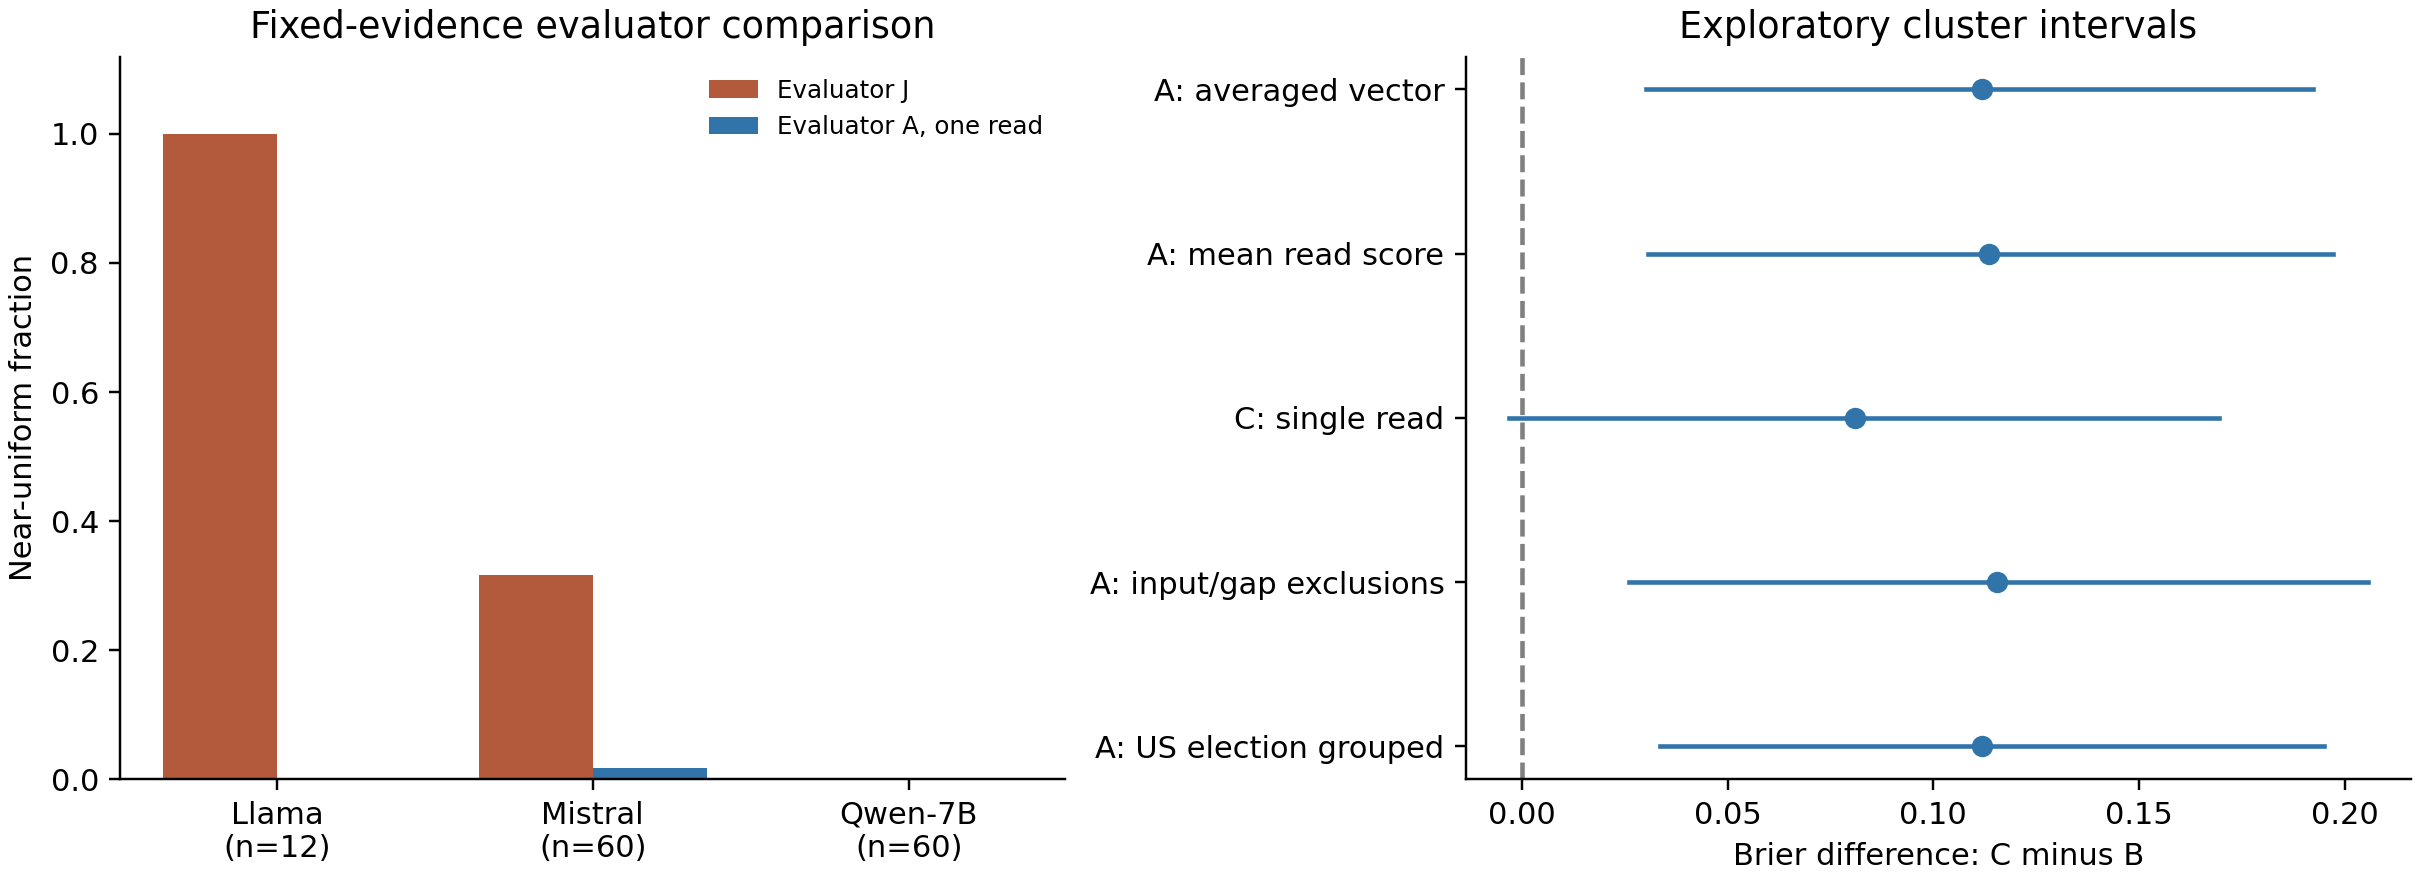
\includegraphics[width=\textwidth]{fig_paper_audit.png}
\caption{Left: fixed-evidence near-uniform counts expressed as fractions
(Table~\ref{tab:paired}). Right: exploratory Brier contrasts under alternative
extraction and clustering choices (Table~\ref{tab:sensitivity}). Bars on the
left are observed fractions, not independent-agent estimates. Intervals on the
right account for repeated campaigns within events; the grouped row additionally
joins six US-election events.}
\label{fig:audit}
\end{figure*}

\subsection{Repeatability within the replacement evaluator}
\begin{table}[!htbp]
\centering
\caption{Evaluator A repeatability across 90 units per campaign.
Reads are available files; four stale file--unit readings are excluded.
Exact agreement concerns probability vectors, not rounded Brier values.}
\label{tab:noise}
\begin{tabular}{lrrr}
\toprule
Campaign & Reads & Exact & Mean BS range\\
\midrule
\NoiseRows
\bottomrule
\end{tabular}
\end{table}

Table~\ref{tab:noise} shows substantial variability in repeated extraction.
Mean within-unit Brier ranges are 0.208--0.375. Repeated reads here are repeated
requests through the recorded deployment, not independent evaluators and not
new simulations. The archive does not establish whether stochastic decoding,
retries, backend nondeterminism or provider routing generated each difference.
Because some requests failed and their stale copies are excluded, read counts
are not perfectly balanced even within a campaign. The ranges support reporting
repeatability alongside forecast quality; they do not provide a universal
noise floor or an optimal number of required reads.

\section{Source Audit and Existing Mechanism Probes}
\label{sec:mechanism}
\subsection{What the code establishes}
The archived client includes a keyword-based bypass for model identifiers
containing strings such as \texttt{r1} or \texttt{reasoning}, and a separate
local-quantization bypass. The identifier \texttt{deepseek-r1-14b} matches
the reasoning filter. This documents a path that disables constraints for the
configured name. Complete historical request logs are unavailable, so actual
constraint status cannot be independently verified for every July request.

Schema enforcement and semantic correctness are different properties.
JSON-object mode guarantees neither the nested schema nor meaningful probabilities.
A schema-valid vector can be uniform, incorrect or unrelated to the transcript.
Evaluator A used JSON-object handling; Evaluator C's strict-schema requests were
documented as falling back after schema rejection. Neither is a verified,
uniformly strict schema-enforced reference instrument.

Silent defaults complicate diagnosis. Historical validation could accept
incomplete micro-question mappings and fill them with missing-value labels.
A deployed normalization path could also replace non-positive matched mass
with a uniform vector. The final probabilities do not consistently preserve
the raw completion and retry history needed to assign the origin of every
uniform vector. The observations cannot establish that uniformity was a
deliberate hedge by the model.

\subsection{Cross-evaluator transfer}
An existing follow-up sent Mistral's 60 simulated evidence records to five
additional unconstrained deployments. The stored experiment reports 8 near-uniform
outputs among 58 parsed Qwen3-14B responses~\cite{qwen3}; six of these eight occur among the
19 units that Evaluator J flattened. Other deployments report zero near-uniform
outputs among 56 DeepSeek-R1~\cite{deepseekr1}, 54 DeepSeek-R1-Distill-Llama-70B,
57 Qwen3-32B~\cite{qwen3}
and 60 Ministral-14B responses.

These are counts among usable responses, not success rates over all attempted
calls. Missing responses cannot be assumed missing at random. The simplified
transfer prompt differs from the production rubric; an additional DeepSeek-R1
production-prompt control reports zero near-uniform outputs among 60 scored units.
This control does not make every cross-model comparison configuration-matched.
The overlap identifies inputs on which two deployments return the same diagnostic
pattern. It does not establish a model-size boundary: size, training and serving
are not independently varied.

\subsection{Truncation and requested enforcement}
\label{sec:truncation_grid}
The existing grid varies four evidence lengths and whether output constraints
are requested for a hosted Qwen3-14B proxy. Truncation retains parts of the log
and subsamples representative actions; it changes content and speaker coverage
together with character count. The original Evaluator J deployment was not
available for this experiment.

\begin{table}[!htbp]
\centering
\caption{Qwen3-14B grid: near-uniform/usable readings out of 60 attempted units
per cell. On denotes requested enforcement; actual strict-schema acceptance
is not verified for every response.}
\label{tab:truncation}
\begin{tabular}{lrr}
\toprule
Length target & Off & On\\
\midrule
\TruncationRows
\bottomrule
\end{tabular}
\end{table}

The unconstrained shortest arm has 7/59 near-uniform readings and the full arm
1/60. Pairing the 59 units with both responses yields six short-only near-uniform
outcomes and zero full-only outcomes. Shortening did not reduce near-uniformity
in this proxy experiment. A descriptive association between longer evidence and
near-uniformity in the original Mistral/J observations cannot be promoted to
a demonstrated length mechanism.

Across all lengths there are 238 matched off/on pairs because missing units
differ between arms. We average paired indicator differences within each event
and resample the 30 events, preserving conditions and length levels. The
equal-event off-minus-on estimate is approximately $+0.005$, with interval
$[-0.029,+0.042]$. The marginal totals, 12/239 and 11/239, should not be treated
as independent binomial samples. This experiment does not detect a clear effect
of requesting enforcement; it neither proves equivalence nor establishes that
enforcement has no effect in the original deployment.

These probes bound candidate explanations without identifying the cause of
Evaluator J's outputs. The extraction-sensitivity observation does not require
either a length mechanism or a schema mechanism to be true.

\section{Exploratory Forecasting Results}
\label{sec:forecast}
\subsection{Post-release subset}
The 20 selected events yield 80 campaign--event records per simulation condition.
Under Evaluator A's averaged vector, B accuracy is \PooledAccuracy\%, comprising
65 outright correct modal outcomes and one two-way tie credited by one half.
The mean uniform-choice reference is 32.6\%. These are descriptive statistics
of retrospective pipeline outputs.

\begin{table}[!htbp]
\centering
\caption{Post-release subset, 20 events per campaign. Accuracy uses tie credit;
Brier uses Evaluator A's averaged vector. Labels do not imply matched serving.}
\label{tab:forecast}
\begin{tabular}{lrrrr}
\toprule
Campaign & Acc.\ B & Acc.\ C & BS B & BS C\\
\midrule
\ForecastRows
\bottomrule
\end{tabular}
\end{table}

The contrast $BS_C-BS_B$ is positive when B scores better.
Table~\ref{tab:sensitivity} presents all sensitivity summaries selected for this
retrospective reanalysis; none is a preregistered hypothesis test.

\begin{table*}[!htbp]
\centering
\caption{Exploratory sensitivity of $BS_C-BS_B$. Intervals resample events,
except the US-election-grouped row (15 clusters over 20 events). Input/gap
exclusion removes C6, T6, T8 and C9 from all campaigns. Exclusions were chosen
after inspection of the audit trail; intervals do not correct for this selection.}
\label{tab:sensitivity}
\begin{tabular}{lrl}
\toprule
Analysis & Events & Mean [95\% interval]\\
\midrule
\SensitivityRows
\bottomrule
\end{tabular}
\end{table*}

The averaged-vector and mean-read-score summaries under A are similar here,
so the B/C estimate is not solely a vector-ensembling artifact. Excluding the
input/gap events retains a positive estimate. Grouping or omitting six
US-election events also retains a positive estimate under A. These checks
do not remove every shared cause of event outcomes.

Evaluator C gives $\EvaluatorCBrier$, whose interval includes zero. Its
single-read budget differs from A's repeated-read budget. This is limited
robustness across the available measurement choices, not a clean test that
one evaluator detects an effect and another does not. A statistical difference
between the two effects is not established.

\subsection{What the contrast cannot identify}
\label{sec:leakage}
The post-release filter concerns the campaign models, not all LLMs in the
pipeline. Evaluators deployed in 2026 may know the outcomes of events from
2024--2025. The probability prompt exposes identifiable questions, and
instructions to use only the discussion do not demonstrate compliance.
Dossiers and perturbations were assembled retrospectively; timestamps, source
fidelity and freedom from hindsight were not independently established for
every claim. Stripping URLs or softening deterministic language cannot remove
knowledge already encoded in a model.

The accuracy figures therefore do not establish leakage-free forecasting.
They may reflect genuine evidence use, pre-existing model knowledge, evaluator
knowledge, retrospective input construction, or a combination. Ground-truth
labels are used as recorded; this study does not independently adjudicate
every market resolution or the mutual exclusivity of every curated option set.

The B/C contrast describes sensitivity of the complete simulated-and-extracted
pipeline to its input conditions. It cannot attribute that sensitivity specifically
to agent-to-agent deliberation. A direct call, an extractor reacting to a changed
transcript, or different injected wording may also produce a B/C difference.
Relevance is not isolated from length, and C6/T6/T8 do not implement the intended
relevance manipulation.

\section{Existing Single-Agent Baseline}
\label{sec:cot}
The post-campaign baseline contains 240 calls: 20 events, four hosted model arms
and three calls per event/arm. Each receives the seed dossier and nominal B
update, not the simulation transcript. The first call uses temperature zero,
the other two temperature 0.7; these are not identically distributed replicates.

The principal summary averages individual-call Brier scores. It estimates
the mean score of the observed three-setting mixture, not a fixed-temperature
single-call policy. The script also reports the first call alone and the score
of the three-vector ensemble. No added retrieval step was executed: the dossier
and injection were supplied directly in the prompt.

Only Llama-3.1-8B and Qwen2.5-7B have nominal model identities matching their
campaigns; identical served weights are not independently verified, and
serving and precision are not fully matched. Ministral-8B~\cite{ministralcards} and Qwen3-14B differ
from the Mistral-7B and Qwen2.5-14B campaigns and are secondary comparisons.

\begin{table*}[!htbp]
\centering
\caption{Existing CoT baseline. Positive $BS_{\rm CoT}-BS_{\rm swarm}$ favours
the swarm. Identity matching does not imply serving/precision matching.
Per-arm intervals are exploratory event bootstraps.}
\label{tab:cot}
\begin{tabular}{lcrl}
\toprule
CoT arm & Identity matched? & Accuracy & Brier difference [95\% interval]\\
\midrule
\CotRows
\bottomrule
\end{tabular}
\end{table*}

Pooling the identity-matched arms by event gives
$BS_{\rm CoT}-BS_{\rm swarm}=\MatchedCotBrier$. The point estimate favours CoT
and the interval includes zero. This is no demonstrated swarm advantage in
the available comparison, not proof of equivalence or non-inferiority.
Some individual or ensemble variants exclude zero in CoT's favour; these
are exploratory and do not change that scope.

Across all four, partly unmatched arms, individual-call accuracy is
\CotAccuracy\%, compared with \PooledAccuracy\% for the swarm under A's
averaged vectors. This does not establish equal capability: model identity,
serving and aggregation are unbalanced. There is no single-agent C arm.
A factorial comparison of single-agent versus simulation crossed with the
same B/C inputs would be needed to estimate additional content sensitivity
from deliberation. The present data do not identify that interaction.

\section{Implications and Limits}
\label{sec:limitations}
\subsection{A practical measurement protocol}
A reproducible evaluation should preserve the event question, ordered options,
evidence bytes, full prompt, model identifier, serving revision when available,
generation parameters, requested and accepted output format, raw completion,
retry history and probability post-processing. A final vector and an error
flag are insufficient to diagnose the defects found here.

Repeated extraction and a second evaluator are useful diagnostics, not substitutes
for external validity. Read counts should follow a precision/cost analysis;
this study does not justify a universal minimum of three reads. A labelled
synthetic transcript or blinded human reference can test extraction fidelity.
A question-only baseline can measure what a later evaluator knows without
the simulation. These are recommendations, not experiments executed in this
revision. Repairing a schema bypass is sound engineering even when its effect
on near-uniformity is unknown. Valid JSON, a non-uniform forecast and a faithful
interpretation are separate requirements.

\subsection{Limits of the evidence}
The primary comparison is conditional on a selected artifact set and a historical
deployment. The original endpoint's disappearance prevents exact intervention
on that deployment. An open-weight model identifier exists, but restoring
weights under a new stack would be a new experiment, not a proven replay.

Repeated reads condition on one realised simulation per condition and cannot
estimate simulation-run variability. Nominally 300 agents sharing a model do
not supply 300 independent replications. The 30-event convenience catalogue
supports limited generalization to other events, languages, forecasting horizons
and deployments.

The seven-dimension rubric, convergence telemetry and persona/action audits
remain execution diagnostics, not validated measures of psychological or
collective-reasoning constructs. Incomplete telemetry, placeholders and serving
failures prevent the original convergence and optimal-configuration claims
from being retained as results. Isolated failures of small deployments do not
establish a general parameter-count exclusion rule.

No causal mechanism is rescued by an insignificant comparison, and an inability
to reject a null is not proof of equality. The main finding is sensitivity of
measured probabilities to extraction configuration; forecasting comparisons
make its consequences and limits visible.

\section{Conclusion}
On 132 matched simulated evidence records, the original and replacement
extraction configurations produce 31 and one near-uniform forecasts. Repeated
reads of the replacement also vary substantially. These observations warrant
treating an LLM extractor as part of the forecasting system.

The source audit and proxy experiments do not identify why the original
configuration produced these vectors or which reading is faithful to the
swarm. Forecasting contrasts remain retrospective, evaluator-dependent and
affected by imperfect inputs. An existing single-agent baseline does not
demonstrate a deliberation benefit. The contribution is a reproducible audit
of extraction sensitivity and the design boundaries it exposes, rather than
a validated advantage or failure of collective reasoning.

\clearpage
\appendices
\section{Experimental and Benchmark Design}
\label{sec:full_design}

\subsection{Taxonomy and Event Selection}
\label{sec:taxonomy}
ECN-BENCH curates 30 resolved categorical questions from Polymarket. Market prices are not a competitive baseline in this experiment. Recorded outcomes are used as supplied, not independently re-adjudicated. The analysed set is defined by the 30 IDs actually present in each campaign, not the superseded counts in the catalogue header.

The initial specification used information type and forecast horizon as design axes. Some catalogue entries contain such metadata. The historical analyses instead used the prefix partition below, which mixes subject matter and question format; it is retained for traceability, not as a validated taxonomy. The extended numerical appendix gives the actual questions, recorded outcomes and all per-event scores.

\begin{table}[!htbp]
\centering
\caption{ECN-BENCH Event Taxonomy as Realised in the 30-Event Corpus}
\begin{tabular}{llcc}
\toprule
\textbf{Prefix} & \textbf{Category} & \textbf{Events} & \textbf{Option count $K$} \\
\midrule
C & Social/Electoral   & 15 & 3--9 \\
S & Senate/Binary      &  7 & 2--4 \\
T & Technical/Economic &  8 & 2--5 \\
\midrule
  & \textbf{Total}     & \textbf{30} & \textbf{2--9} \\
\bottomrule
\end{tabular}
\label{tab:taxonomy}
\end{table}

\subsection{Experimental Conditions}
The implemented conditions are listed below. They do not isolate a causal effect of deliberation because the direct reference is shared and the B/C controls are imperfect:
\begin{itemize}
    \item \textbf{Condition A (shared direct reference):} Seed-based reference evidence is reused across campaigns. This is not an independently executed baseline for each campaign model.
    \item \textbf{Condition B (nominally relevant injection):} A configured 300-agent, 60-round simulation receives an event-specific update at round 30. Seven injection IDs target a stale catalogue; relevant is therefore the intended rather than universally realised manipulation.
    \item \textbf{Condition C (null injection):} The same configured workflow receives an unrelated administrative message at round 30. Null payloads repeat the same body and are not length-matched to the B payloads.
\end{itemize}

\subsection{Simulation Output Fidelity: Action Density and Scope Conditions}
\label{sec:action_fidelity}

The original project reported a cluster-side scan of 1,380 SQLite database files. The two tables preserve that historical scan, including sweeps and wrong-topic Qwen2.5-14B executions; they are not a matched comparison of the four currently scored campaigns. The complete original collection is no longer available for rechecking. A cursor-tracking issue in actions summaries can omit organic actions during telemetry rounds without removing them from the SQLite trace table.

\begin{table}[!htbp]
\centering
\caption{Historical Cluster-Scan Social-Action Counts from SQLite Trace Tables (1,380 Database Files, Mixed Campaigns and Sweeps). The \texttt{actions.jsonl} summary files undercount organic actions due to a cursor-tracking bug during telemetry-probe rounds (see text); the \texttt{.db} files are the authoritative source.}
\label{tab:action_density_30event}
\small
\begin{tabular}{lcccc}
\toprule
\textbf{Model} & \textbf{DBs} & \textbf{Total Social} & \textbf{Avg/DB} & \textbf{Agent Traces} \\
 & \textbf{scanned} & \textbf{Actions} & & \\
\midrule
Llama-3.1-8B-AWQ  & 672 & \textbf{27,087} & \textbf{40.31} & 554,782 \\
Mistral-7B-Instruct-v0.1    & 264 & 9,364           & 35.47          & 257,339 \\
Qwen2.5-14B   & 180 & 2,407           & 13.38          & 113,366 \\
Qwen2.5-7B-GGUF   & 264 & 723             & 2.74           & 191,942 \\
\bottomrule
\end{tabular}
\smallskip \\
\footnotesize ``Social Actions'' = post + comment + like + comment\_like + follow + dislike + comment\_dislike (excluding telemetry probes and refresh/sign\_up). ``Agent Traces'' = all trace-table rows including telemetry. Llama-3.1-8B's 672 DBs include the main July campaign (180) plus optimization sweeps and earlier runs; per-DB averaging normalizes across unequal DB counts. Qwen2.5-14B's 180 DBs = a reported 30-event execution collection (30 events $\times$ 3 conditions $\times$ 2 platforms). \textbf{Reproducibility caveat:}  these counts were obtained by SQL queries executed on the cluster and are not recoverable from the released \texttt{event\_results.json} artifacts, which do not carry action counts. They could not be re-verified during the audit described in Appendix~\ref{sec:data_audit} and are reported on the authority of the original scan. Exporting per-unit action counts into the released summaries is a required change for the next campaign. Note also that the Llama-3.1-8B row pools heterogeneous configurations (different $N$ and $R$ across sweeps), so its per-DB average is not directly comparable with rows drawn from a single fixed configuration.
\end{table}

\begin{table}[!htbp]
\centering
\caption{Social-Action Breakdown by Type (Historical .db Scan, Mixed Campaigns and Sweeps).}
\label{tab:action_breakdown}
\small
\begin{tabular}{lcccc}
\toprule
\textbf{Action} & \textbf{Llama-8B} & \textbf{Mistral-7B} & \textbf{Qwen-14B} & \textbf{Qwen-7B} \\
\midrule
post             & 8,079  & 4,476  & 1,215 & 592 \\
comment          & 5,421  & 1,978  & 585   & 108 \\
like             & 4,567  & 1,946  & 461   & 16  \\
comment\_like    & 3,010  & 167    & 124   & 1   \\
follow           & 5,993  & 708    & 11    & 1   \\
dislike          & 7      & 67     & 0     & 5   \\
comment\_dislike & 10     & 22     & 11    & 0   \\
\midrule
\textbf{Total}   & \textbf{27,087} & \textbf{9,364} & \textbf{2,407} & \textbf{723} \\
\bottomrule
\end{tabular}
\setlength{\tabcolsep}{6pt}
\end{table}

Action counts do not establish deliberation quality, antagonism, human-like cognition or causal forecasting mechanisms. Unequal execution collections cannot rank campaigns. The original all-campaign scan is distinct from the run-integrity audit and the currently scored evidence; in particular, its Qwen2.5-14B row includes executions against subsequently corrected questions.


\section{The Seven-Dimension Grading Framework}
\label{sec:grading}

This section restores the complete seven-dimension design specification. It is not a psychometrically validated scale or seven successfully measured outcomes. Probability-vector Brier scores are recomputed; the remaining dimensions require observables and construct validation that the campaign does not consistently supply. Original weights and display bands document the intended protocol, not empirically justified weights.

\subsection{D1: Prediction Accuracy (Weight: 0.25)}
The primary forecasting metric is the \textbf{Multi-Category Brier Score ($BS$)}, which evaluates the extracted probabilistic forecast. For a given event with $K$ mutually exclusive categories, let $f_k$ be the swarm's predicted probability for category $k$, and $o_k$ be the one-hot indicator of the realized outcome ($o_k = 1$ if category $k$ occurred, $0$ otherwise). The Brier Score is formulated as:
\begin{equation}
    BS = \sum_{k=1}^K (f_k - o_k)^2
\end{equation}
The unnormalised multicategory Brier score lies in $[0,2]$. A correct deterministic forecast attains zero; a deterministic forecast on one wrong option attains two. Uniform probability scores $1-1/K$ for every outcome. Brier measures overall probabilistic performance, not calibration alone. All current scores are recomputed from vectors rather than inherited scalar fields.

The aggregate Brier Score across $E$ events is $BS_c = \frac{1}{E} \sum_{e=1}^E BS_{e,c}$ for condition $c \in \{A, B, C\}$. 

We formally define \textbf{Simulation Lift ($Lift$)} as the historical difference in Brier score:
\begin{equation}
    Lift = BS_A - BS_B
\end{equation}
A positive value means B scores lower than the shared A reference. It is not a within-model simulation effect, even if an interval excludes zero. Evaluator identity and input provenance remain part of the comparison. The principal observable input contrast is $BS_C-BS_B$, with its remaining confounds stated explicitly.

The specification also proposes Brier skill relative to a uniform vector. For pooled reporting, averaging eventwise ratios differs from dividing mean Brier by mean reference; the aggregation must be specified. The main paper uses unnormalised Brier with equal event weights rather than claiming normalization removes all outcome-space effects:
\begin{equation}
    BSS = 1 - \frac{BS_{model}}{BS_{random}} \quad \text{where} \quad BS_{random} = 1 - \frac{1}{K}
\end{equation}
Where $BS_{random}$ represents the expected multi-category Brier error under uniform random guessing ($f_k = \frac{1}{K}$). The BSS metric possesses intuitive econometric bounds:
\begin{itemize}
    \item $BSS = +1.0$: Perfect deterministic prediction ($f_{correct} = 1.0$).
    \item $BSS = 0.0$: Performance equivalent to uniform random guessing.
    \item $BSS < 0.0$: Sub-random performance (worse than uninformed guessing).
\end{itemize}
The specified display score is $D1_{\mathrm{score}}=\max(0,100\,BSS_B)$. Clipping hides differences below the reference and is not itself a proper scoring rule. It is retained as an interface convention, not used for inference or model selection.

\subsection{D2: Polarization (Weight: 0.15)}
The construction below is inspired by Esteban and Ray~\cite{esteban1994}; its vector-valued extension and clustering choices are specific to the benchmark proposal.
To measure whether the agent swarm fragments into deeply entrenched, opposing camps, we utilize the \textbf{Esteban-Ray (ER) Index of Polarization}. Rather than measuring general dispersion, the ER Index captures both identification (internal group cohesiveness) and alienation (distance between groups). Assume the simulated population forms $G$ distinct opinion clusters regarding the event outcome. Let $p_i$ be the population proportion of cluster $i$, and $y_i$ be the mean probability vector of group $i$. The ER Index is defined as:
\begin{equation}
    ER(\alpha) = \kappa \sum_{i=1}^G \sum_{j=1}^G p_i^{1+\alpha} p_j \|y_i - y_j\|_1
\end{equation}
Where:
\begin{itemize}
    \item $\alpha$ is the polarization sensitivity parameter. The protocol selects $\alpha=1.0$; this is not an empirically calibrated psychological parameter.
    \item $\kappa$ is a normalization constant scaling $ER \in [0, 1]$.
    \item The clustering procedure and normalization must be specified before computing this index.
\end{itemize}
This functional increases with separation under its chosen clustering, distance and normalization. Its vector-valued extension and nominal score $S_2=100(1-ER_{\mathrm{norm}})$ are protocol choices. A reproducible implementation requires an explicit clustering rule and normalization; a generated high/low label is not a measured real-population polarization index.

\subsection{D3: Herd Effect (Weight: 0.15)}
The proposed herd diagnostic counts changes in modal answers toward the majority. This is a behavioral transition statistic, not a causal measure of social pressure: shared evidence, common model priors and a moving majority can generate the same pattern. The original indicator is:
\begin{equation}
    Conform_{i,t} = \mathbf{1}\left[\text{argmax}_k p_{i,t,k} = M_t \quad \text{and} \quad \text{argmax}_k p_{i,t-1,k} \neq M_{t-1}\right]
\end{equation}
The raw herd index for a simulation is:
\begin{equation}
    Herd = \frac{1}{T \cdot N_{agents}} \sum_{t=1}^T \sum_{i=1}^{N_{agents}} Conform_{i,t}
\end{equation}
The proposed B/C contrast is:
\begin{equation}
    D3_{raw} = Herd_B - Herd_C
\end{equation}
Neither this sign nor a raw count separates mimicry from rational updating. A strong response to relevant information may be appropriate. Computing the indicator requires longitudinal agent probabilities and a tie convention, not a substitute evaluator impression.

\subsection{D4: Deliberation Quality (Weight: 0.15)}
The conceptual source is the discourse-quality framework of Steenbergen et al.~\cite{steenbergen2003}; the shortened LLM rubric is an adaptation, not a validated reproduction of that instrument.
The design adapts discourse-quality ideas into the criteria below. It originally targeted a stratified sample of 100 interactions; the surviving evidence uses a capped, ranked sample instead. This is not proof that 100 random interactions were evaluated for every unit:
\begin{enumerate}
    \item \textbf{Participation:} Equality and accessibility of speech acts.
    \item \textbf{Level of Justification:} Whether claims are accompanied by logical assertions ($0$: no justification; $1$: inferior; $2$: qualified; $3$: sophisticated).
    \item \textbf{Respect:} Tone toward peers ($0$: disrespectful; $1$: neutral; $2$: explicitly respectful).
    \item \textbf{Constructive Politics:} Collaboration toward a consensus ($0$: positional; $1$: alternative proposals; $2$: mediating consensus).
\end{enumerate}
The normalized score is $S_4 = 100 \times \frac{Score_{observed} - Score_{min}}{Score_{max} - Score_{min}}$.

\subsection{D5: Susceptibility (Weight: 0.10)}
The proposed susceptibility measure contrasts pre/post Brier changes in B and C. It requires valid pre-injection probabilities on the same outcome space and matched measurement at both times. These formulas specify the intended quantity, not an estimand established by final-output records alone:
\begin{equation}
    PostImprove_{e,m,c} = BS_{e,m,c, (t=29)} - BS_{e,m,c, (t=60)}
\end{equation}
Where $t=29$ is the step immediately preceding the perturbation. The raw Susceptibility score is the difference in lift:
\begin{equation}
    D5_{raw} = \frac{1}{E} \sum_{e=1}^E \left(PostImprove_{e,m,B} - PostImprove_{e,m,C}\right)
\end{equation}
A positive value describes a larger measured score improvement in B conditional on valid measurements. It does not mathematically establish rationality or noise resistance. The current analysis uses the observable final-output contrast and does not invent round-29 measurements.

\subsection{D6: Convergence (Weight: 0.10)}
DeGroot's linear opinion-pooling model~\cite{degroot1974} motivates the notation; the LLM simulation has not been shown to obey that model.
We model consensus formation through the \textbf{DeGroot Consensus Model}. In the classical model, agent beliefs evolve via a transition probability matrix $W$ representing social trust, such that $x(t+1) = W x(t)$. In ECN-BENCH, we measure the mathematical distance to consensus by the final round. First, we define the dispersion trajectory of agent probability vectors at step $t$:
\begin{equation}
    Disp_t = \frac{1}{N_{agents}(N_{agents}-1)} \sum_{i < j} \sum_{k=1}^K |p_{i,t,k} - p_{j,t,k}|
\end{equation}
The opinion convergence (contraction rate) is defined as:
\begin{equation}
    Contr = 1 - \frac{Disp_{T}}{Disp_{1}}
\end{equation}
To prevent the swarm from converging on the wrong answer (i.e., highly confident but incorrect consensus), we implement an \textbf{Accuracy Guard}:
\begin{equation}
    Guard = 1 - BS_B
\end{equation}
The convergence score is formulated as the joint product:
\begin{equation}
    D6_{raw} = \text{mean}_e (Contr_e \times Guard_e)
\end{equation}
Under the adopted convention, $1-BS_B$ ranges from $-1$ to $1$, not $0$ to $1$. The contraction ratio is undefined at zero initial dispersion and may be negative. The original dispersion sum is over $i<j$ but divided by $N(N-1)$, yielding half the mean unordered-pair distance; consistent scaling cancels in its ratio. Incomplete telemetry does not validate this composite.

\subsection{D7: Information Diversity (Weight: 0.10)}
The diversity component proposes entropy over semantic argument bins. Its interpretation depends on an explicit binning and coding procedure, not the number of agents. The released categorical judgments do not establish that a reproducible semantic-binning procedure was executed:
\begin{equation}
    H = - \sum_{i=1}^S q_i \ln(q_i)
\end{equation}
To normalize this across varying bin sizes, we compute Pielou's Evenness (Shannon Equitability):
\begin{equation}
    E_H = \frac{H}{\ln(S)}
\end{equation}
The intended aggregate is $S_7=100\,\mathrm{mean}_{e,t}E_{H,e,t}$. Zero-frequency terms contribute zero. A single bin requires an explicit convention because $\ln S=0$, and an empty sample is missing rather than maximally diverse. Diversity alone is not accuracy or independent information.

\subsection{Composite Aggregation and Grade Bands}
The final \textbf{ECN-Predictability Index (EPI)} is a weighted composite of the seven normalized dimension scores ($S_1 \dots S_7 \in [0, 100]$):
\begin{equation}
    EPI = 0.25 S_1 + 0.15 S_2 + 0.15 S_3 + 0.15 S_4 + 0.10 S_5 + 0.10 S_6 + 0.10 S_7
\end{equation}
The resulting $EPI$ was intended to map to the project-defined display bands, as defined in Table~\ref{tab:grades}.

\begin{table}[!htbp]
\centering
\caption{Original Proposed Display Bands (Not Validated Academic Grades)}
\begin{tabular}{lcl}
\toprule
\textbf{EPI Range} & \textbf{Grade} & \textbf{Interpretation} \\
\midrule
90 - 100 & A+ & Exceptional multi-agent forecasting and dynamic deliberation \\
80 - 89  & A  & Strong, well-calibrated, and resilient swarm intelligence \\
70 - 79  & B  & Solid performance, with minor miscalibrations or conformity issues \\
60 - 69  & C  & Mixed/unstable quality; susceptible to noise \\
50 - 59  & D  & Weak simulation lift; poor deliberation quality \\
$<$ 50   & F  & Fails baseline forecasting expectations \\
\bottomrule
\end{tabular}
\label{tab:grades}
\end{table}


The EPI requires seven valid normalized inputs. Missing or unstable dimensions cannot be silently filled with zeros or uniform buckets, nor dropped while retaining the original interpretation. No EPI ranking is reported. Rubric repeatability is a diagnostic, not construct validation.



\section{Full Protocol, Estimands and Measurement Boundaries}
\label{sec:full_protocol}
\subsection{Original research questions and their operational limits}
ECN-BENCH was designed around three questions: whether simulation improves a direct forecast, whether agent beliefs converge, and whether relevant information changes beliefs differently from a null update. These questions remain part of the research programme. The audit distinguishes them from what the released measurements identify.

The direct-forecast question requires an independently executed baseline for each campaign model, with comparable inputs, serving and evaluation. A shared reference does not implement that comparison. The convergence question requires valid longitudinal probabilities and a defined distance between distributions; a generated rubric label or a constant initialized telemetry series does not implement it. The information-response question requires interpretable B/C inputs. The recorded injection bank changes length and diversity as well as intended relevance, and includes wrong-topic inputs. None of these conditions can be repaired retrospectively by changing a statistical test.

The configured 300 agents and 60 rounds are properties of the execution design. They are not 300 independent forecast replications and do not enlarge the event sample. Three hundred model-generated personas may share priors, errors, textual templates and a serving endpoint. Their effective information content is not determined by their nominal count.

\subsection{Graph memory, persona generation and context controls}
\label{sec:confound}
The intended pipeline builds an event context, generates personas, executes social actions, stores memory and extracts probabilities from a digest. Graph-building and evaluation models were intended to remain fixed across comparisons. That is a design goal rather than a demonstrated property of every original and recovery request. Role names in a configuration are insufficient: the actual endpoint, model identifier, library revision and fallback route should be recorded.

Graph-based retrieval and temporal memory are infrastructure choices. GraphRAG~\cite{graphrag2024} addresses corpus-level question answering through graph indexing and summarization; it does not establish that the present implementation improves forecasting. A functioning Neo4j instance likewise does not prove that agents retrieved relevant memory or that a retrieved fact was historically available at the forecast date. Separating memory construction from the campaign model is useful for experimental control, but introduces another potentially knowledgeable LLM component.

The original context-sanitization protocol removed URLs, rewrote resolution contracts and softened statements about likely outcomes. Those steps may make prompts more consistent; they do not erase model knowledge or establish a historical information barrier. Retrospectively authored dossiers can contain hindsight without explicitly naming the eventual outcome. The term gold-standard context is therefore withdrawn as a validation claim.

\subsection{Why the original inferential arguments are not retained}
\label{sec:statistics}
\label{sec:power_limitation}
A sample mean is a valid descriptive statistic even when squared errors are not normally distributed. Distributional assumptions matter for inference about a population, not for reporting the mean of an observed dataset. The earlier assertion that empirical means are statistically invalid is withdrawn.

For paired losses $d_e=L_A(e)-L_B(e)$, the familiar statistic
\[
t_d=\frac{\overline d}{s_d/\sqrt{E}}
\]
uses event pairs, not agents, as observations. It does not address a shared-reference design defect or evaluator leakage. Calling it a Diebold--Mariano statistic without specifying the forecast sequence and long-run variance does not establish time-series validity. In this catalogue, apparently separate questions can share one underlying event, particularly the 2024 US election. An arbitrary event order is not a justified autocorrelation structure.

Observed power computed from the measured effect size largely restates the same test statistic. The earlier combination of incompatible power formulas, an asserted 92-event requirement, and agent-level binomial margins of error is not retained. The illustrative independent-pair normal approximation,
\[
E_{\mathrm{approx}}=\left(
  \frac{z_{1-\alpha/2}+z_{1-\beta}}{d_z}
\right)^2 ,
\]
would give approximately 32 independent pairs for $d_z=0.5$, two-sided $\alpha=0.05$ and target power 0.8. This arithmetic is not a sample-size recommendation for ECN-BENCH: it omits event dependence, run variability, selection and uncertainty in the assumed effect. No further runs were selected or scheduled using it.

The old pooled accuracy test has a separate problem. Four campaigns answering the same question do not supply four independent event outcomes, and a tie-aware total such as 65.5 is not an integer binomial count. Rounding it upward does not produce an exact Poisson-binomial test for the reported estimand. Its very small numerical value is withdrawn, not merely re-labelled exploratory.

\subsection{The implemented event-cluster bootstrap}
The current computation first averages each event's contrast across the four fixed campaigns, then resamples events. It uses 100,000 percentile draws with generator seed 7. The US-election sensitivity instead resamples 15 clusters containing 20 events, preserving equal-event weighting when cluster sizes differ. Repeated readings and campaigns belonging to the same sampled event remain together. Resampling agents or evaluator rows independently would manufacture replication.

These intervals quantify variability of the observed event-level contrasts under the chosen resampling scheme. They do not include an unobserved distribution of simulation seeds, future questions, provider configurations or unseen evaluators. Grouping six election questions is a sensitivity analysis, not proof that every remaining event is independent. Neither an interval including zero nor a non-significant comparison proves equivalence.

\subsection{Scoring, ties, sharpness and calibration}
A uniform forecast is included in all score summaries. For a binary event that resolves yes, $(0.5,0.5)$ scores 0.5, whereas $(0,1)$ scores 2. A reduction in confidence can therefore improve or worsen Brier depending on the outcome and the starting distribution. There is no general rule that a flatter forecast mechanically increases loss relative to another forecast.

Sharpness is a property of the predictive distribution without reference to the realized outcome. The probability assigned to the outcome is not a definition of sharpness. Modal confidence is the maximum forecast probability; directional accuracy asks whether its maximizers include the outcome, with fractional tie credit. The regenerated confidence bins use these two quantities consistently. They do not bin on the known outcome's probability and then claim to measure top-label calibration.

An empirical reliability diagram with only a few events per bin is descriptive. It cannot establish that a model is calibrated on a future population, and a cell with two successes in two events is not proof of perfect calibration. No calibration transformation was fitted on these same outcomes and then presented as out-of-sample performance.

\subsection{Reference scores, format effects and mathematical coupling}
A uniform Brier reference depends on the option count $K$. Normalizing each event before averaging changes its relative weight compared with an unnormalised mean. The report retains the original BSS definition as a protocol option, but does not call uniform probability a competitive baseline or describe BSS as eliminating all difficulty differences between binary and multicategory questions.

The earlier difficulty--lift plot contains a shared term: its axes are $A$ and $A-B$, where $A=BS_A$ and $B=BS_B$. In general,
\[
\operatorname{Corr}(A,A-B)=
\frac{\operatorname{Var}(A)-\operatorname{Cov}(A,B)}
{\sigma_A\sqrt{\operatorname{Var}(A)+\operatorname{Var}(B)-2\operatorname{Cov}(A,B)}}.
\]
Even if $A$ and $B$ are independent, this becomes
$\sigma_A/\sqrt{\sigma_A^2+\sigma_B^2}$, which can be large.
That coupling does not prove that every observed association is meaningless; it shows why a large correlation alone is not evidence of an informative event-selection rule. A weak correlation between $A$ and $B$ in a small selected sample also does not prove that baseline difficulty has no predictive value.

The historical SBE/SDE labels classify observed score differences after the fact. They are retained in the figure register as names used during investigation, not as independently validated event classes. Selecting events on low $BS_A$ or large $BS_A-BS_B$ cannot then be used as independent evidence that the same score-defined class benefits from simulation.

\subsection{Aggregation budgets and the single-agent estimand}
A mean probability vector is a forecast ensemble. Its Brier score differs from the mean score of its members by the mean squared vector dispersion. The report exposes both quantities rather than describing repeated reads as a way to recover a uniquely true swarm forecast. Exact vector agreement is strict, while a within-unit score range grows with the number of available reads; neither supplies a universal measurement threshold.

The existing CoT experiment supplied a dossier and an injection directly, not a newly executed retrieval pipeline. Its three calls use a temperature-zero setting followed by two temperature-0.7 settings. Mean individual-call score estimates the observed mixture of settings, while the three-vector ensemble is a different forecast with a different budget. The two nominally matched model arms are not verified identical-serving comparisons. Without a single-agent C arm, the deliberation-by-input interaction is not identified.



\section{Extended Source-Code and Extraction Audit}
\label{sec:source_extended}
\subsection{The micro-question channel}
\label{sec:epistemic_mapping}
The benchmark's epistemic-mapping proposal asks event-specific micro-questions in addition to a macro forecast. A response contains a dominant tag and a short rationale intended to connect transcript content to a granular event driver. This channel is distinct from both the categorical forecast and the seven rubric dimensions; correctness in one field does not validate the others.

The historical manuscript described widespread missing mappings, often stored as \texttt{N/A} with a missing-response rationale. Such a record can result from a validator filling an omitted field rather than a model explicitly returning that judgment. Missingness should be counted by the actual keys and responses in a specified file. The earlier expression $3\times270\times3=2430$ is not a valid count for three micro-questions across 270 already model-indexed units: it counts the campaigns twice. No current result relies on that aggregate.

The earlier 63-run pilot inventory distinguished provider-style identifiers from local served-model names. Naming is suggestive, not a verified endpoint trace, and those pilot runs change model, prompt, serving and task configuration together. Their reported local/cloud split is a historical troubleshooting observation, not a controlled experiment establishing a deployment-location effect.

\subsection{Schema bypass and runtime provenance}
A client branch tests model-name substrings including \texttt{r1} and \texttt{reasoning}. The configured original evaluator name matches that test. The source also contains a local-quantization branch. These are inspectable control paths, not behavioral hypotheses about a model's intelligence.

The snapshots are not interchangeable. The newer client in
\path{07_pipeline/backend/app/utils/llm_client.py} and the deployment snapshot
in \path{09_audit/source_snapshots/hpc_llm_client.py}
document differing constraint and fallback policies. Full request logs and a serving-revision ledger would be needed to assign a precise policy to every historical call. It is therefore incorrect to infer from one current source snapshot that every July request had exactly the same accepted response format.

JSON syntax, nested schema membership and semantic fidelity are separate properties. A schema can require probabilities for all options and still admit a uniform vector. Constraints cannot prohibit hedging unless a task-specific rule explicitly does so, and prohibiting uniform probability would not make the forecast truthful. The original assertion that enforcement forecloses a uniform hedge is withdrawn. The observed J/A difference is a configuration contrast, not a verified intervention on this branch alone.

\subsection{Retry, validation and silent defaults}
The probability evaluator historically checked some required mappings before accepting a response, but a missing micro-question could be backfilled after that check. A top-level successful call therefore does not imply a complete semantic response. A retry may also alter temperature or feedback, so a final accepted vector need not be a sample from the nominal first-attempt policy.

The older \texttt{hpc\_evaluator.py} normalization path coerces or drops some invalid values and can return uniform probability when matched mass is non-positive. The newer source rejects that case. The archived snapshot and its SHA-256 make this distinction independently inspectable; neither establishes which individual historical uniform vectors were produced by normalization rather than by the model.

A robust record should retain raw output, the parsed object, option matching, pre-normalization mass, validation exceptions, every retry and the final decision. Final vectors and completion flags alone cannot identify all failure origins. This is why the paper calls near-uniformity an output diagnostic rather than declaring every such unit a failed forecast.

\subsection{Separating predictions from derived metrics}
A re-evaluation utility can replace probabilities while leaving stored Brier, ranked probability score, directional accuracy and calibration fields untouched. Such a file can be syntactically valid and scientifically inconsistent. The historical reconciliation step separated evaluator datasets rather than overwriting one pass with another. The current analysis goes further by recomputing the metrics used in the paper directly from each vector.

A scalar must be stored with the hash or version of the prediction from which it was derived. Catalogue identity likewise requires more than an event ID. Two questions may share a yes/no option set and the same recorded outcome, so option/outcome validation cannot catch every topic collision. The surviving Qwen2.5-14B T1 mismatch is a concrete example.

\subsection{Pairing after recovery}
The original local evaluator cannot have evaluated newly generated recovery evidence before that evidence existed. Llama's replaced units and Qwen2.5-14B's repaired rows are therefore not included as J observations merely because their filename is \texttt{event\_results.json}. The primary paired audit is restricted to the 132 B/C units whose historical configurations read matching evidence, questions, ordered options and outcomes.

Those checks establish equality of the retained inputs, not equality of complete HTTP requests, micro-question prompts, retry histories or generation settings. The evaluator names are archived execution identifiers; the report does not guarantee current provider routing or weight identity. A repeat call with the same configured seed can still differ under a changed or nondeterministic backend.

\subsection{Existing transfer and truncation controls}
The transfer experiment uses one campaign's evidence and different deployed evaluators under a simplified prompt. Its parsed-response denominators differ. It cannot be treated as a complete-case success rate over all attempted calls, nor as an isolated test of model size. The production-prompt control is useful but does not retroactively match every other configuration.

The truncation grid alters retained content, action selection and speaker coverage together with length. Requested enforcement is not confirmed strict-schema acceptance for every response. The 238 complete off/on pairs are nested within events and lengths, not independent binomial trials. The absence of a clear pooled effect in this proxy does not prove that constraints never matter or identify the original J mechanism. These existing probes are fully reported without adding evaluator calls.

\section{Run Integrity, Persona Realization and Evidence Coverage}
\label{sec:full_campaign_supporting}
\subsection{How the evidence categories differ}
This appendix restores the detailed operational context behind the short-form findings. It separates four kinds of evidence: frozen vectors reanalysed by executable code; retained source and logs that document a failure path; historical summary scans whose full input collection no longer survives; and mechanistic interpretations that remain untested. Only the first supports the regenerated forecast tables. Historical scan tables are retained as labeled records, not promoted to new matched-campaign results.

\subsection{Persona pools versus configured population}
\label{sec:persona_audit}
A configured population is an upper bound on the number of distinct persona descriptions, not a measured cognitive sample size. The original pre-repair audit counted persona strings, fallback biographies and literal four-axis labels. Its table is retained below because the failure mode is important: a nominal 300-agent run can be populated largely by repeated templates.
\begin{table*}[!htbp]
\centering
\caption{Historical pre-repair persona-string audit of the three original campaigns. Literal template compliance and distinct strings do not validate cognitive diversity. The Llama row includes subsequently replaced outage records; these are not statistics of its recovered campaign.}
\label{tab:persona_audit}
\footnotesize
\setlength{\tabcolsep}{3pt}
\resizebox{\textwidth}{!}{%
\begin{tabular}{lccccc}
\toprule
\textbf{Campaign} & \textbf{Distinct personas / 300} & \textbf{min / median / max} & \textbf{Boilerplate bio} & \textbf{4-axis compliance} & \textbf{Units $\leq$ 20 distinct} \\
\midrule
Mistral-7B-Instruct-v0.1 & $295.6$ & $263 / 298 / 300$ & $0.7\%$  & $97.7\%$ & $0/90$ \\
Llama-3.1-8B-AWQ         & $71.6$  & $11 / 11 / 271$    & $79.0\%$ & $16.2\%$ & $69/90$ \\
Qwen2.5-7B-GGUF          & $38.0$  & $19 / 40 / 57$     & $92.0\%$ & $1.7\%$  & $9/90$ \\
\bottomrule
\end{tabular}%
}
\setlength{\tabcolsep}{6pt}
\end{table*}

The pre-repair Llama audit describes repeated event-independent archetypes following an endpoint failure. Qwen2.5-7B supplied fewer distinct persona strings than configured agents, while Mistral more often emitted the specified literal axis labels. These are observable formatting and duplication properties. A unique string need not express an independent viewpoint, and a missing literal label need not imply that the corresponding concept is absent. Neither measure supplies a population margin of error.

\subsection{Outage, partial execution and misleading completion flags}
\label{sec:outage}
The run-integrity investigation found a temporal break in the original Llama execution sequence: repeated connection failures, a fallback persona library, few organic actions and missing telemetry interviews. The six unaffected events retained in the J/A audit are C3 and S2--S6. Later recovery replaced 24 event records; the historical shorthand of 23 outage events should not be confused with the size of that replacement set, which also includes a transitional/catalogue correction history.

A successful process exit or an orchestrator status of completed does not establish successful agent inference. The affected historical records can carry \texttt{error: null} and no evaluator-fallback flag while their simulation logs contain repeated endpoint failures. This does not imply that the evaluator itself failed to make a call: the forecast stage may successfully score an error-filled digest of an unsuccessful simulation.

The distinction matters for units such as the historical Llama C10/B record. The original audit describes an evidence field dominated by connection errors and repeated question/injection lines, yet accompanied by probability and rubric outputs. The scientific defect is that a plausible downstream response masks absent upstream discussion. Rubric scores assigned to such material are not evidence that deliberation occurred.

The old all-campaign action inventory includes parameter sweeps and pre-repair runs. The narrower post-repair scan below is a different collection. Neither can be substituted for the other or used as a controlled model comparison; in particular, the original ranking changed when the execution collection changed.
\begin{table*}[!htbp]
\centering
\caption{Reported post-repair action-count scan for the three 30-event execution collections. Counts describe stored action types, not semantic quality; these historical scan totals are not regenerated by the probability reanalysis. Telemetry interviews are not substantive social posts.}
\label{tab:action_30event_only}
\small
\begin{tabular}{lcccccc}
\toprule
\textbf{Campaign} & \texttt{create\_post} & \texttt{create\_comment} & \texttt{follow} & \texttt{like\_post} & \texttt{like\_comment} & \texttt{interview} \\
\midrule
Llama-3.1-8B-AWQ         & $\mathbf{9{,}074}$ & $\mathbf{6{,}454}$ & $\mathbf{5{,}046}$ & $\mathbf{4{,}046}$ & $\mathbf{2{,}044}$ & $60{,}000$ \\
Mistral-7B-Instruct-v0.1 & $3{,}545$ & $1{,}648$ & $576$ & $1{,}618$ & $139$ & $60{,}000$ \\
Qwen2.5-7B-GGUF          & $281$ & $104$ & $1$ & $14$ & $1$ & $60{,}000$ \\
\bottomrule
\end{tabular}
\setlength{\tabcolsep}{6pt}
\end{table*}

\subsection{The first recovery merge was also defective}
The first attempted recovery rebuilt records from configuration keys that did not contain the expected question/evidence fields. The recorded problem was not a small numerical discrepancy: evidence could be empty, a condition-insensitive merge could overwrite the shared A reference, and one source could populate nominally distinct evaluator files. Those mistakes created apparent differences between conditions and apparent agreement between evaluators for the wrong reasons.

The corrected recovery rebuilt evidence from available logs/actions, restored the shared reference instead of re-eliciting it, and separated evaluator outputs. It also used a hosted Llama endpoint rather than the original local AWQ deployment. The repair is therefore a replacement execution under a changed serving configuration, not proof that the original local run can be replayed exactly.

A generation budget that succeeds on empty evidence may fail on a full transcript. The historical recovery record reports null completions and increased completion budgets during rescoring. That change is part of the extraction configuration; it must not be hidden behind a single evaluator-model label. The revision adds no recovery execution of its own.

\subsection{Catalogue collisions and the remaining T1 mismatch}
\label{sec:fourth_model_status}
The stale catalogue reused short event IDs for different questions. A downstream micro-question collision and an upstream wrong-topic simulation are different defects. Correcting a micro-question label does not repair a discussion generated for the wrong event, and repairing a discussion does not automatically repair the separate injection bank.

Qwen2.5-14B previously had six wrong-topic events replaced. During restoration of the full per-event tables, a stricter cross-campaign question check identifies a remaining T1 mismatch in all three primary conditions: the other campaigns ask whether the UAW reaches an agreement with the Big Three automakers before November 1, 2023, while Qwen2.5-14B asks about a Fed rate cut in November 2024. The yes/no options and recorded outcome coincide. This is precisely the kind of collision that a probability-simplex or outcome-key check cannot detect.

The full numerical appendix retains the stored T1 rows so the defect is visible, but excludes T1 across all four campaigns from its 29-event aligned summaries and confidence bins. The main 20-event subset already excludes T1, so its estimates are unchanged. No question, vector or simulated evidence was edited to conceal the mismatch. Recovering T1 with another run is not necessary to state the present audit results and has not been attempted.

Qwen2.5-14B C9/C separately retains an outage-like integrity concern. The main paper reports an input/gap sensitivity excluding C9 along with C6, T6 and T8. Alignment of the remaining 29 questions is not certification of simulation health.

\subsection{What survives when raw traces are missing}
Qwen2.5-14B's six recovered events and an original C15 fragment retain raw artifacts. Original raw traces for 21 other events are unavailable following scratch-storage deletion. Scored evidence fields survive, so probability reanalysis and digest inspection remain possible. Persona and database scans requiring the lost originals cannot be reproduced across that entire campaign.

The original Qwen2.5-14B all-campaign SQL scan predates the six question repairs. Its counts include wrong-topic executions; the affected count is six events, not six database files. Event, condition, platform database, request and evaluator-read counts must not be interchanged. The original 180-database inventory is retained as a historical inventory, not reconstructed as if it were the corrected 120 B/C platform databases.

\subsection{Sampled evidence is not the complete conversation}
\label{sec:evidence_depth}
The scored evidence is a digest: a log tail and a representative-action block. A historical sampler ranks actions by a fixed engagement heuristic, selects up to 60 and orders those selections by round. The cap limits what the evaluator sees; it does not make all evidence equally informative or guarantee that every unit reaches the cap. Sparse runs can include telemetry scaffolding instead of substantive utterances.

Probe lines such as a belief check with a missing value are instrumentation artifacts, not independent arguments from a person. Counting distinct speaker labels without examining message content can therefore overstate conversational diversity. Conversely, a small text sample does not establish that the entire underlying simulation was inactive.
\begin{table}[!htbp]
\centering
\caption{Historical digest audit of the then-current scored evidence: proportion of sampled lines identified as telemetry probes. These figures are retained from the original audit record, not recomputed as part of the present probability analysis. Instrumentation content is not automatically outcome leakage.}
\label{tab:probe_share}
\small
\begin{tabular}{lccc}
\toprule
\textbf{Campaign} & \textbf{Probe share} & \textbf{Probe share} & \textbf{Distinct} \\
 & (mean) & (median) & \textbf{utterances} \\
\midrule
Llama-3.1-8B             & $0.0\%$          & $0.0\%$          & $56$ \\
Mistral-7B-Instruct-v0.1 & $0.0\%$          & $0.0\%$          & $41.5$ \\
Qwen2.5-7B-GGUF          & $\mathbf{86.0\%}$ & $\mathbf{86.7\%}$ & $8$ \\
Qwen2.5-14B-AWQ          & $\mathbf{72.0\%}$ & $\mathbf{90.0\%}$ & $6$ \\
\bottomrule
\end{tabular}
\end{table}

Telemetry in the digest is not automatically ground-truth leakage. A valid agent probability probe may be a legitimate part of the input, whereas an invalid placeholder is missing measurement. The methodological problem is that the pipeline did not isolate these channels or consistently distinguish them in its final record. Campaign-level differences in probe share are confounded with model and serving identity, so a pooled correlation cannot identify their effect on accuracy.

Option names can also occur as persona display names. Seeing a candidate's name in a political discussion is not by itself proof that the outcome label leaked: an incorrect option can appear the same way, and all options may be known before resolution. An outcome-aware selection of names would be more serious, but that provenance is not established by an exact string match. The corrected interpretation is a possible cue channel requiring an outcome-blind check, not a demonstrated source of the forecast's accuracy.

\subsection{Two qualitative event readings}
\label{sec:case_studies}
The original close reading contrasted Llama C11, the Nobel Peace Prize question, with S6, the Austrian election question. Those discussions are retained as qualitative diagnostic examples, not a matched causal experiment: S6 is among the unchanged local units and C11 belongs to the recovered hosted execution, so they do not share one serving history.

For C11, the audit described generic social advocacy plus an injection favoring atomic-bomb-survivor organizations. A resulting forecast can react to that cue without demonstrating that agent-to-agent deliberation discovered the outcome. A persona name matching an option is a possible additional prompt cue, not conclusive proof of outcome contamination.

For S6, the sampled discussion was largely about sustainability and other off-topic themes rather than the Austrian election. Fluent agreement in such a sample is not evidence of task-relevant consensus. An extractor assigning mass to a residual option can reflect its interpretation of that sample, its own prior or both.

These examples motivate a distinction between generating conversation and delivering relevant evidence to the extractor. They do not estimate the prevalence of either pattern or locate a general mechanism. Small score differences between a CoT call and a swarm on one chosen event are not equivalence tests. The full per-event numerical tables make the current vector-derived values available without presenting the selected anecdotes as confirmatory results.

\subsection{Rubric repeatability and construct validity}
\label{sec:evaluator_reliability}
The historical rubric compares repeated calls of a deployed evaluator, not independent human raters. Cohen's kappa~\cite{cohen1960} describes label agreement after its marginal adjustment and depends on label prevalence. A low value is a repeatability warning; a high value would still not demonstrate that the labels measure polarization, herding or deliberation quality.
\begin{table}[!htbp]
\centering
\caption{Historical repeated-call rubric agreement values. The operational 0.8 cutoff was a project rule, not a universal validity threshold. Campaign and evaluator revisions are not matched; these figures do not rank model capacity.}
\label{tab:kappa_summary}
\small
\begin{tabular}{lccc}
\toprule
\textbf{Dimension} & \textbf{Llama-3.1-8B} & \textbf{Mistral-7B} & \textbf{Qwen2.5-7B} \\
\midrule
prediction\_accuracy    & 0.321 & 0.182 & 0.088 \\
polarization           & 0.241 & 0.167 & 0.122 \\
deliberation\_quality  & 0.209 & 0.228 & 0.062 \\
herd\_effect           & 0.206 & 0.113 & 0.053 \\
convergence            & 0.245 & 0.139 & 0.212 \\
susceptibility         & \textbf{0.322} & \textbf{0.245} & 0.033 \\
information\_diversity & 0.228 & 0.130 & 0.103 \\
\midrule
\textbf{Max $\kappa$}  & \textbf{0.322} & \textbf{0.245} & \textbf{0.212} \\
\textbf{Dropped dims}  & 7 & 7 & 7 \\
\bottomrule
\end{tabular}
\setlength{\tabcolsep}{6pt}
\end{table}

The project applied a 0.8 operational threshold and dropped unstable dimensions. That threshold is not a universal scientific boundary, and moving to a finer scale does not guarantee greater validity. No EPI composite is restored as an empirical model ranking. The proposed dimension definitions remain available in the technical specification so that future validation can examine them rather than assuming them correct.

\subsection{Telemetry placeholders and the meaning of convergence}
\label{sec:jsd_convergence}
The historical Jensen--Shannon divergence (JSD) audit~\cite{lin1991jsd} found repeated initialization-like values and constant series. A non-increasing series passes a non-strict monotonicity test even when it never changes. It follows that a count of monotonic runs cannot establish convergence without verifying successful probes and understanding what distributions were compared.
\begin{table}[!htbp]
\centering
\caption{Historical telemetry integrity summary, before recovery: 60 B/C units and 600 checkpoints per campaign. The last column counts decreasing transitions out of 540, not converging runs. Constant initialization values cannot establish convergence.}
\label{tab:convergence_jsd}
\small
\begin{tabular}{lccccc}
\toprule
\textbf{Model} & \textbf{Mean} & \textbf{Pipeline} & \textbf{Placeholder} & \textbf{Constant} & \textbf{Strictly} \\
 & \textbf{JSD} & \textbf{``monotonic''} & \textbf{values} & \textbf{series} & \textbf{decreasing} \\
\midrule
\textbf{Llama-3.1-8B-AWQ} & 0.734 & 48 & 526/600 (87.7\%) & 48/60 & 29 \\
\textbf{Mistral-7B-Instruct-v0.1}   & 0.637 & 0  & 244/600 (40.7\%) & 0/60  & \textbf{133} \\
\textbf{Qwen2.5-7B-GGUF}  & 0.628 & 0  & 166/600 (27.7\%) & 0/60  & \textbf{113} \\
\bottomrule
\end{tabular}
\smallskip\\
\footnotesize ``Placeholder values'' counts checkpoint readings exactly equal to $0.758277$, the constant the telemetry emits when no probed distribution is available. ``Constant series'' counts units whose ten checkpoint values are all identical. ``Strictly decreasing'' counts round-to-round transitions with a JSD decrease exceeding the pipeline tolerance $\epsilon = 0.002$, out of 540 transitions per model.
\end{table}

The pipeline's JSD construction also needs to be distinguished from inter-agent disagreement. A distance between an aggregated histogram and a fixed uniform reference is not the same as pairwise belief dispersion, and neither is automatically a distance to a correct consensus. A decline can reflect a changing reference relationship, aggregation or placeholder behavior rather than increasing agreement among agents. A valid DeGroot interpretation requires additional structure not measured here.

\subsection{Topology, behavior and limits of interpretation}
The historical run manifest records an unspecified default degree distribution rather than a measured power law. The previously asserted exponent is withdrawn. A directed complete graph has at most $N(N-1)$ non-self edges; that bound is not the realized edge count, message volume or memory load in this sparse execution.

Follows, replies, likes and dislikes describe selected tool actions. They do not identify antagonism, reflective cognition or a causal epistemic mechanism without content validation and controlled comparison. A low follow count does not make topology irrelevant, because an initial graph or recommendation mechanism may still expose posts. Nor does agreement across campaigns prove shared memorization or social amplification.

Interventions such as forced posting, reply requirements or diversity penalties would change the simulated process. They may be useful future experiments but are not repairs that can be assumed to preserve the original estimand. No such intervention was run in this revision.

\subsection{Temporal exposure and the retained event subsets}
\label{sec:contamination}
\label{sec:cutoff}
A low baseline Brier score can result from an easy dossier, base rates, fortunate confidence, genuine inference or prior knowledge. Thresholding that score does not identify training contamination. It also selects on a component of the lift statistic, so a lift reversal after removing low-baseline-score events is partly a consequence of the selection rule.

Release dates are a more externally defined descriptive stratifier, but the forecast is produced by the whole pipeline. Later extractors may know outcomes, and retrospectively authored inputs can expose them. A post-release label for a campaign checkpoint is therefore not a certificate that the observed pipeline forecast was made under genuine future uncertainty.

The retained 20-event set is listed in the main analysis. Six entries share the US election and are grouped or omitted in sensitivity checks. Three contain wrong-topic injections and C9 carries a further integrity concern. The unchanged primary comparison should be read with all these qualifications, rather than selecting whichever evaluator or subset gives the strongest interval.


\section{System Architecture and Engineering (MiroFish-Offline)}
\label{sec:architecture}

The historical execution stack was designed for restricted-network HPC environments. The architecture below describes the intended pipeline and engineering revisions, not a claim that every campaign completed all steps successfully. Original and recovered runs do not share one immutable stack.

\begin{figure*}[!tbp]
\centering
\begin{tabular}{|c|}
\hline
\textbf{Step 1: GraphRAG Build} \\
$\downarrow$ \\
\textbf{Step 2: Persona Generation (4-Axis DNA, Neo4j Graph Memory)} \\
$\downarrow$ \\
\textbf{Step 3: 60-Step OASIS Simulation (MiroFish-Offline Engine)~\cite{yang2024,oasissoftware,mirofishoffline}} \\
$\rightarrow$ \textit{Step 30: Nominally Relevant vs. Unrelated Injection} \\
$\downarrow$ \\
\textbf{Step 4: Output Extraction (Telemetry Logging \& Actions DB)} \\
$\downarrow$ \\
\textbf{Step 5: ReportAgent Extraction (Versioned Evaluator Configuration)} \\
$\downarrow$ \\
\textbf{Step 6: Scoring \& Statistical Inference (Brier and Proposed Behavioral Diagnostics)} \\
\hline
\end{tabular}
\caption{The ECN-BENCH Multi-Agent Social Simulation Pipeline.}
\label{fig:pipeline}
\end{figure*}

\subsection{The Local Serving Stack}
The project's original compute jobs used restricted-network nodes, motivating local services. This is a constraint of the recorded environment, not a claim that every university cluster prohibits outbound access. Hosted recovery and post-campaign evaluator calls are separately identified. The intended local components were:
\begin{itemize}
    \item \textbf{Primary Inference Server:} vLLM~\cite{vllm} hosted open-weight models. Its continuous batching and PagedAttention support batched serving; the archived jobs record the deployment-specific vLLM configuration rather than implying portability across versions.
    \item \textbf{Embedding Server:} The archived release implements an Ollama endpoint~\cite{ollamasoftware} hosting \texttt{nomic-embed-text} for vector-similarity queries. The Nomic model card~\cite{nomiccard} documents the model family; the archived alias does not preserve an exact version or revision. No Infinity dependency or import is present in the released source, so Infinity is not claimed as an executed component.
    \item \textbf{Graph Engine:} A self-hosted Neo4j Community Edition instance and project-specific Neo4j storage/retrieval code manage graph state. No Graphiti dependency or import is present in the archived release, so this report does not attribute the implementation to Graphiti.
\end{itemize}

\subsection{HPC Scalability Migration (Architecture v5.0 - v5.10)}
Scaling and concurrent telemetry exposed routing, container and storage bottlenecks. The following changes document the engineering response. They reduced specific failure risks; the later outage shows that they did not establish absolute stability.

\subsubsection{Hybrid LLM Routing (v5.0)}
The original routing experiment separated chat generation from embedding service load. Primary interaction could use vLLM on port 8000 while embedding requests used a separate service on port 11434. This is a workload-isolation choice, not a general claim that Ollama lacks batching or cannot serve concurrent requests.

\subsubsection{Multi-GPU Server Isolation (v5.5)}
To support 100-agent simultaneous telemetry probes without stalling the social simulation, a 4-GPU isolation protocol was established:
\begin{itemize}
    \item \textbf{Benchmark Server (GPUs 0,1):} Handles active agent interactions (Post/Reply/Like) on Port 8000.
    \item \textbf{Evaluator/Telemetry Server (GPUs 2,3):} Dedicated to probability probing and final scoring on Port 8001.
\end{itemize}
This separation reduces direct resource contention; it does not guarantee immunity to timeouts, queue saturation or shared-node failures. Actual GPU assignments must be read from each job rather than inferred from this reference layout.

\subsubsection{Apptainer Containerization (v5.6 - v5.7)}
The project used Apptainer/Singularity containers, including a recorded vLLM 0.6.3-based image, to reduce host-environment variation. Experimental bind mounts replaced selected Python packages when the image lacked support for a checkpoint. The illustrative mount below is an engineering record, not a guaranteed reproducible environment: a changed library tree alters the software revision even when the container image name is unchanged.
\begin{equation}
    \begin{split}
    \text{Bind Mount Target: } -B \; &\text{\texttt{/scratch/waves/transformers}} \\
    :\,&\text{\texttt{/usr/local/lib/python3.12/}} \\
     &\text{\texttt{dist-packages/transformers}}
    \end{split}
\end{equation}
This replaces the immutable container libraries at runtime with development versions, adjusting for Python 3.12 container environments while the host runs Python 3.11.

\subsubsection{NFS Database Concurrency and Waves NVMe Migration}
The project encountered SQLite lock errors on network-backed storage during concurrent activity. Two recorded mitigations were a longer connection timeout and relocation of active data to node-local scratch. These can reduce contention but do not eliminate all locking errors or guarantee transaction safety:
\begin{enumerate}
    \item \textbf{The Connection Lock Protocol:} All SQLite connectors enforce a strict 60-second queue timeout:
    \begin{verbatim}
    sqlite3.connect(database_path, timeout=60)
    \end{verbatim}
    \item \textbf{Waves NVMe Relocation:} Neo4j graph data and active \texttt{.db} files are symlinked directly onto local high-I/O scratch spaces (\texttt{/scratch/waves/} NVMe drives), reducing network-storage latency without guaranteeing absence of lock contention.
\end{enumerate}



\subsection{Reproducibility costs of mutable environments}
A container digest, bind-mounted package tree, model weights, tokenizer and serving flags jointly define the execution environment. A container tag alone is insufficient. Recovery via a hosted endpoint can restore usable evidence without restoring the original hardware, numerical precision or routing behavior. The release therefore separates analysis reproducibility from replay of the complete historical system.

Scratch relocation also creates a retention risk. The missing Qwen2.5-14B originals show that successful execution is not a preservation strategy. Source data should be exported before ephemeral storage expires; manifests and checksums should describe what was actually exported, including partial coverage. This report does not claim that missing raw artifacts have been reconstructed.



\section{Complete Scaling and Computational-Cost Record}
\label{sec:results}
The original scaling campaign is retained as an engineering exploration rather than removed from the report. It examined two anchor questions, C1 and C9, using one run per configuration/condition. No new sweep was run for this revision. The original numerical matrices below are retained as historical execution records; the current probability-analysis scripts do not claim to regenerate their full execution history.

\subsection{Population sweep}
\label{sec:n_scaling}
At 60 rounds, the population settings were 30, 100, 300, 1,000 and 3,000 agents. The table supports a non-monotone description, not a fitted scaling law. On C1 the lowest observed B score is at 100 agents; on C9 it is at 30, not in the previously claimed 100--300 optimal zone. At 1,000 agents, C9 scores below its 300-agent value, while C1 scores above it. Those facts contradict a universal monotonic degradation story.
\begin{table}[!htbp]
\centering
\caption{Historical single-run population sweep at 60 rounds. Each cell is an observed execution record, not a population estimate; no replicated uncertainty is available.}
\label{tab:n_sweep_results}
\begin{tabular}{lcccccc}
\toprule
 & \multicolumn{3}{c}{\textbf{Event C1: US Election}} & \multicolumn{3}{c}{\textbf{Event C9: UK Trade}} \\
\cmidrule(r){2-4} \cmidrule(l){5-7}
\textbf{$N$ (agents)} & \textbf{Cond A} & \textbf{Cond B} & \textbf{Cond C} & \textbf{Cond A} & \textbf{Cond B} & \textbf{Cond C} \\
\midrule
30      & 0.3368 & 0.5300 & 0.4200 & 0.2150 & 0.5952 & 0.6069 \\
\textbf{100}     & 0.3368 & \textbf{0.3958} & 0.5958 & 0.2150 & 0.6971 & 0.6329 \\
\textbf{300}     & 0.3368 & 0.5350 & 0.6800 & 0.2150 & 0.7630 & 0.8197 \\
1000    & 0.3368 & 0.9533 & 0.9000 & 0.2150 & 0.7264 & 0.6417 \\
3000    & 0.3368 & 0.6133 & 0.7911 & 0.2150 & 0.7885 & 0.6095 \\
\bottomrule
\end{tabular}
\setlength{\tabcolsep}{6pt}
\end{table}
The theoretical upper bound $N(N-1)$ on directed non-self links is not the realized number of graph edges or messages. A complete graph at 3,000 agents would have many potential links, but the deployed interaction policy is not a complete communication network. Neither memory saturation nor collapsing signal-to-noise was directly measured by these Brier cells. A uniform distribution also maximizes, rather than minimizes, Shannon entropy~\cite{shannon1948}, so an earlier low-entropy uniform-weight argument is mathematically incorrect.

\subsection{Round sweep}
\label{sec:r_scaling}
At 300 agents, the recorded round settings were 30, 60 and 90. C1 Brier falls from 0.7200 to 0.5350 and then rises to 0.9983. C9 changes from 0.7721 to 0.7630 to 0.7850. The much smaller C9 differences cannot be treated as independent confirmation of a sharp collapse boundary. With one realization per cell, between-run variability is unknown.
\begin{table}[!htbp]
\centering
\caption{Historical single-run round sweep at 300 agents. A change in Brier does not establish convergence or locate an echo-chamber threshold.}
\label{tab:r_sweep_results}
\begin{tabular}{lcccccc}
\toprule
 & \multicolumn{3}{c}{\textbf{Event C1: US Election}} & \multicolumn{3}{c}{\textbf{Event C9: UK Trade}} \\
\cmidrule(r){2-4} \cmidrule(l){5-7}
\textbf{$R$ (rounds)} & \textbf{Cond A} & \textbf{Cond B} & \textbf{Cond C} & \textbf{Cond A} & \textbf{Cond B} & \textbf{Cond C} \\
\midrule
30  & 0.3368 & 0.7200 & 0.6283 & 0.2150 & 0.7721 & 0.7386 \\
\textbf{60}  & 0.3368 & \textbf{0.5350} & 0.6800 & 0.2150 & \textbf{0.7630} & 0.8197 \\
90  & 0.3368 & 0.9983 & 0.6958 & 0.2150 & 0.7850 & 0.8401 \\
\bottomrule
\end{tabular}
\setlength{\tabcolsep}{6pt}
\end{table}
Sixty rounds yield a lower observed Brier than the other two round settings on these two anchors. That is not a proof that agent beliefs converge by rounds 40--50 or that an echo chamber starts at rounds 70--80. The telemetry integrity issues independently prevent that interpretation. The negative A-to-B contrast on C1 is not a positive lift merely because B improves between round settings.

\subsection{Why 300 agents and 60 rounds were selected}
\label{sec:optimal_bounds}
\label{sec:optimal_config}
The production configuration is a pragmatic historical choice balancing execution cost, space for persona diversity and the observed anchor-event scores. It is not an empirically established optimum. The claim that 300 generated agents provide a binomial 95\% margin of error of 0.056 assumes independent observations of a common population quantity that these correlated language-model personas do not supply. That agent count also has no direct role in the event-level bootstrap denominator.

Distinct persona strings must be measured, and four conceptual axes do not partition 300 agents into four independent samples of 75. The persona audit shows why nominal capacity and realized variety differ. A larger configured population can increase resource demand without increasing independent task-relevant information.

The configuration should therefore be interpreted as an execution parameter held nominally fixed in the main campaigns. A new choice would require a prespecified utility/cost objective and replicated measurements under the intended workload. This report neither recommends another production setting nor launches the simulations needed to evaluate one.

\subsection{Cross-model anchor checks}
\label{sec:cross_model}
The anchor comparisons retain model-specific reference values and unbalanced coverage. Qwen2.5-14B has only C1 in this particular matrix; that is not its coverage in the separate recovered 30-ID campaign. A missing C9 cell is not zero and should not be filled from a different campaign.
\begin{table*}[!htbp]
\centering
\caption{Historical anchor-event campaign comparison at the selected configuration. Model, serving, precision and reference construction are not matched. These are not a validated ranking or a universal optimum.}
\label{tab:cross_model_results}
\begin{tabular}{llcccccc}
\toprule
 & & \multicolumn{3}{c}{\textbf{Event C1: US Election}} & \multicolumn{3}{c}{\textbf{Event C9: UK Trade}} \\
\cmidrule(r){3-5} \cmidrule(l){6-8}
\textbf{Model} & \textbf{Role} & \textbf{Cond A} & \textbf{Cond B} & \textbf{Cond C} & \textbf{Cond A} & \textbf{Cond B} & \textbf{Cond C} \\
\midrule
Llama-3.1-8B-AWQ  & Reference  & 0.3368 & 0.5350 & 0.6800 & 0.2150 & 0.7630 & 0.8197 \\
Qwen2.5-7B    & Validation & 0.5600 & \textbf{0.4450} & 0.6217 & 0.2150 & 0.6080 & 0.7209 \\
Qwen2.5-14B   & Validation & 0.5600 & 0.5978 & 0.5958 & ---   & ---   & ---   \\
Mistral-7B-Instruct-v0.1    & Validation & 0.5600 & 0.6600 & 0.6333 & 0.2150 & 0.8286 & 1.1037 \\
\bottomrule
\end{tabular}
\setlength{\tabcolsep}{6pt}
\end{table*}
The positive Qwen2.5-7B A-to-B contrast on C1 and negative contrasts in other cells are descriptive. They do not demonstrate that one architecture benefits from deliberation and another saturates before 60 rounds. Model generation, serving and precision differ, and no replicated factorial experiment separates those factors.

\subsection{Runtime and resource accounting}
\label{sec:runtime_breakdown}
Each recorded event job contains setup, reference/persona work, simulation B, simulation C and evaluator-related work. The original table separates phase durations and total scheduler wall-clock time.
\begin{table}[!htbp]
\centering
\caption{Historical single-event C1 wall-clock record on the recorded A100 deployment. Job duration includes setup and teardown; it is not GPU-hours, token cost or a throughput guarantee.}
\label{tab:runtime_breakdown}
\footnotesize
\setlength{\tabcolsep}{4pt}
\begin{tabular}{lcccc}
\toprule
\textbf{Model} & \textbf{Phase A (Persona Gen+Eval)} & \textbf{Sim B (With-Sim)} & \textbf{Sim C (Null)} & \textbf{Wall-Clock Total} \\
\midrule
Llama-3.1-8B-AWQ  & 3.8 min (229s)   & 35.1 min (2104s) & 31.4 min (1883s) & 77.6 min (4655s) \\
Qwen2.5-7B    & 2.7 min (161s)   & 47.9 min (2874s) & 18.4 min (1103s) & 77.1 min (4624s) \\
Qwen2.5-14B   & 2.7 min (160s)   & 69.5 min (4168s) & 31.5 min (1890s) & 114.0 min (6842s) \\
Mistral-7B-Instruct-v0.1    & 2.7 min (160s)   & 33.7 min (2024s) & 30.1 min (1806s) & 75.4 min (4526s) \\
\bottomrule
\end{tabular}
\smallskip \\
\footnotesize Each row reflects a single-event (C1) three-condition run from the July 2026 v523 optimization sweep at $N=300$, $R=60$ on \texttt{A100}. ``Wall-Clock Total'' is the Slurm job wall time and includes setup/teardown overhead, so phase times need not sum exactly to it. LLM persona generation alone is approximately $49$\,s ($0.8$\,min); the remainder of Phase A ($\sim$110--180\,s) is persona evaluation and scoring.
\end{table}
A wall-clock minute is not a GPU-minute unless the allocation is one GPU for that entire interval. Idle reservation, parallel services, retries and differently sized allocations matter. The phase durations need not sum to the scheduler total, and the table does not establish a general linear cost law or a monetary price. Earlier conversions from these wall-clock values into campaign-wide GPU-hour requirements are not retained.

A configuration with lower observed loss and longer runtime can be preferable under one utility function and worse under another. Even on C1, 60 rounds cannot be called Pareto-dominant over 30 merely because it has lower Brier: the shorter configuration may cost less. No population cost-performance frontier is established by two selected questions with no repeated runs.

\subsection{Hardware routing and deployment failures}
\label{sec:small_model_limits}
The historical log discusses initialization failures on older GPU nodes, context-window overflow, KV-cache allocation errors and persona JSON parsing failures. These are distinct failure classes. A configured maximum context of 4,096 versus a prompt needing more space is an interface-budget problem; increasing it can increase memory demand. A memory-utilization flag is a fraction of a deployment's available resources, not a portable capacity threshold.

The original troubleshooting settings of 8,192 maximum tokens and memory fractions 0.40 or 0.45 document particular attempts, not guaranteed minimums for other hardware, batch sizes, tokenizers or serving revisions. The recorded A100 scheduling constraint addressed the local deployment; it is not a claim that every older GPU is incapable of every operation required by the pipeline.

Guided-decoding compilation, schema mismatch and invalid unconstrained content also require separate diagnosis. The fact that two small Gemma-family deployments failed does not identify a 15B parameter boundary, an architectural impossibility, or a general incompatibility of all AWQ checkpoints. Successful smaller deployments elsewhere in the same project already make such a universal claim untenable.

\subsection{Revised configuration decision record}
\begin{table*}[!htbp]
\centering\small
\caption{What each configuration consideration can and cannot establish. This replaces the original decision matrix's unvalidated precision and echo-chamber labels.}
\begin{tabular}{p{0.20\textwidth}p{0.32\textwidth}p{0.37\textwidth}}
\toprule
Consideration & Observable in this record & Not established\\
\midrule
Agent count & Configured slots; recorded persona strings & Independent sample size or cognitive coverage\\
Round count & Executed horizon and single-run score & Consensus time or collapse threshold\\
Brier & Loss of the extracted probability vector & Truthfulness of its interpretation of the swarm\\
Runtime & Deployment-specific elapsed duration & Portable GPU-hours, price or general scaling law\\
Schema handling & Source branches and some response records & Semantic correctness or universal prevention of uniformity\\
Model size & Identity of attempted deployments & A sub-15B exclusion rule\\
\bottomrule
\end{tabular}
\end{table*}

\section{Extended Follow-Up Programme}
\label{sec:extended_future_work}
These items restore the original future-work scope while separating proposals from completed experiments. None was executed or scheduled in this revision.

\begin{enumerate}
\item \textbf{Extraction fidelity:} construct outcome-blind reference transcripts or obtain blinded human judgments of what the discussion supports. This would distinguish a different extractor from a more faithful one.
\item \textbf{Evaluator prior knowledge:} compare question-only, dossier-only and transcript-conditioned extraction with versioned prompts. This requires additional calls, not necessarily new simulations, and would still not by itself certify freedom from leakage.
\item \textbf{Deliberation contribution:} cross single-agent versus simulation with matched B/C inputs and model/serving conditions. Repeated simulation seeds would be needed to study between-run stability.
\item \textbf{Input integrity:} version/hash catalogue questions, ordered options, dossiers and injection bodies. Treat topic mismatches as invalid pairings, not as values to repair silently after analysis.
\item \textbf{Telemetry integrity:} retain successful and failed probe counts, missingness and raw probability vectors. Exclude invalid checkpoints from convergence measurements rather than assigning a numeric default.
\item \textbf{Persona and graph realization:} measure distinct descriptions, realized topology and task-relevant information flow. Do not equate string diversity with cognitive independence.
\item \textbf{Scaling:} define a cost/loss objective before comparing replicated settings on new questions. The two existing anchors are exploratory design inputs, not a validation set.
\item \textbf{Artifact preservation:} export ephemeral storage, preserve raw completions and record accepted schema status, retry history and model/serving revisions.
\end{enumerate}

The first two items are particularly relevant to extending the extraction claim; the third is needed for a stronger claim about deliberation itself. None is required to report the current fixed-evidence configuration observation with its stated limitations. Increasing the number of runs simply to obtain a smaller $p$-value is not a justified follow-up strategy.

\clearpage
\section{Complete Event Register and Regenerated Numerical Tables}
\label{sec:full_tables}
\label{sec:per_event_tables}
\subsection{Complete question and outcome register}

Recorded outcomes are reproduced for audit, not independently adjudicated. Post-release denotes the retained date-based subset, not freedom from evaluator knowledge. Wrong injection identifies the known stale-bank topic mismatch.

\paragraph*{C1} Which party will win the 2024 US Presidential Election?

\begin{itemize}

\item Recorded outcome: Republican.

\item Ordered options: Republican; Democrat; Other.

\item Post-release subset: yes; wrong-topic injection: no.

\end{itemize}

\paragraph*{C2} Who will be the 2024 Democratic presidential nominee?

\begin{itemize}

\item Recorded outcome: Harris.

\item Ordered options: Biden; Harris; Newsom; Michelle Obama; Other.

\item Post-release subset: no; wrong-topic injection: no.

\end{itemize}

\paragraph*{C3} Which party wins the most seats in the 2024 French snap legislative election?

\begin{itemize}

\item Recorded outcome: Nouveau Front Populaire.

\item Ordered options: Rassemblement National; Nouveau Front Populaire; Ensemble; Other.

\item Post-release subset: no; wrong-topic injection: no.

\end{itemize}

\paragraph*{C4} Which party will win the most seats in the 2024 UK general election?

\begin{itemize}

\item Recorded outcome: Labour.

\item Ordered options: Labour; Conservative; Reform UK; Other.

\item Post-release subset: no; wrong-topic injection: no.

\end{itemize}

\paragraph*{C5} What will be the balance of power after the 2024 US election?

\begin{itemize}

\item Recorded outcome: Republican President + Republican Congress.

\item Ordered options: Republican President + Republican Congress; Republican President + Split Congress; Democratic President + Democratic Congress; Democratic President + Split Congress; Other.

\item Post-release subset: yes; wrong-topic injection: no.

\end{itemize}

\paragraph*{C6} Which geographic origin will the next Pope elected in the 2025 Papal Conclave come from?

\begin{itemize}

\item Recorded outcome: North American Cardinal.

\item Ordered options: Italian / European Cardinal; Latin American Cardinal; African Cardinal; North American Cardinal; Asian or Other Cardinal.

\item Post-release subset: yes; wrong-topic injection: yes.

\end{itemize}

\paragraph*{C7} Which country will win the 2024 UEFA European Championship?

\begin{itemize}

\item Recorded outcome: Spain.

\item Ordered options: Spain; England; France; Germany; Portugal; Other.

\item Post-release subset: no; wrong-topic injection: no.

\end{itemize}

\paragraph*{C8} Which AI company will first release a model scoring >90\% on MMLU?

\begin{itemize}

\item Recorded outcome: OpenAI.

\item Ordered options: OpenAI; Google DeepMind; Anthropic; Meta; Other.

\item Post-release subset: yes; wrong-topic injection: no.

\end{itemize}

\paragraph*{C9} Which countries will the US agree trade deals with before July 2025?

\begin{itemize}

\item Recorded outcome: UK.

\item Ordered options: UK; India; Japan; Vietnam; South Korea; EU; Canada; Mexico; Other / None.

\item Post-release subset: yes; wrong-topic injection: no.

\end{itemize}

\paragraph*{C10} Who will be the next UK Prime Minister after the 2024 election?

\begin{itemize}

\item Recorded outcome: Keir Starmer.

\item Ordered options: Keir Starmer; Rishi Sunak; Nigel Farage; Other Conservative; Other.

\item Post-release subset: no; wrong-topic injection: no.

\end{itemize}

\paragraph*{C11} Who will win the 2024 Nobel Peace Prize?

\begin{itemize}

\item Recorded outcome: Nihon Hidankyo.

\item Ordered options: Nihon Hidankyo; Pope Francis; UN Agency; Individual Activist; Other.

\item Post-release subset: yes; wrong-topic injection: no.

\end{itemize}

\paragraph*{C12} Which team will win the 2024 NBA Championship?

\begin{itemize}

\item Recorded outcome: Boston Celtics.

\item Ordered options: Boston Celtics; Oklahoma City Thunder; Denver Nuggets; Minnesota Timberwolves; Other.

\item Post-release subset: no; wrong-topic injection: no.

\end{itemize}

\paragraph*{C13} Who will win the 2025 Oscar for Best Picture?

\begin{itemize}

\item Recorded outcome: Anora.

\item Ordered options: Anora; The Brutalist; Conclave; Emilia Pérez; Wicked; Other.

\item Post-release subset: yes; wrong-topic injection: no.

\end{itemize}

\paragraph*{C14} Which party will form the next government after the 2025 German federal election?

\begin{itemize}

\item Recorded outcome: CDU/CSU-led coalition.

\item Ordered options: CDU/CSU-led coalition; SPD-led coalition; AfD-led coalition; Other / Hung parliament.

\item Post-release subset: yes; wrong-topic injection: no.

\end{itemize}

\paragraph*{C15} How many total rate cuts will the Fed deliver in 2024?

\begin{itemize}

\item Recorded outcome: 3.

\item Ordered options: 0; 1; 2; 3; 4; 5+.

\item Post-release subset: yes; wrong-topic injection: no.

\end{itemize}

\paragraph*{S2} Which party will control the US Senate after the 2024 election?

\begin{itemize}

\item Recorded outcome: Republican.

\item Ordered options: Republican; Democrat.

\item Post-release subset: yes; wrong-topic injection: no.

\end{itemize}

\paragraph*{S3} Will Republicans achieve a red sweep in 2024 (Presidency + House + Senate)?

\begin{itemize}

\item Recorded outcome: YES.

\item Ordered options: YES; NO.

\item Post-release subset: yes; wrong-topic injection: no.

\end{itemize}

\paragraph*{S4} Will total 2024 presidential election turnout fall in the 155--160 million bracket?

\begin{itemize}

\item Recorded outcome: YES.

\item Ordered options: YES; NO.

\item Post-release subset: yes; wrong-topic injection: no.

\end{itemize}

\paragraph*{S5} Will the GOP popular vote margin of victory be less than 1.5\%?

\begin{itemize}

\item Recorded outcome: YES.

\item Ordered options: YES; NO.

\item Post-release subset: yes; wrong-topic injection: no.

\end{itemize}

\paragraph*{S6} Which party wins the most seats in the 2024 Austrian legislative election?

\begin{itemize}

\item Recorded outcome: FPÖ.

\item Ordered options: FPÖ; ÖVP; SPÖ; Other.

\item Post-release subset: yes; wrong-topic injection: no.

\end{itemize}

\paragraph*{S7} Will OpenAI become a for-profit company in 2025?

\begin{itemize}

\item Recorded outcome: YES.

\item Ordered options: YES; NO.

\item Post-release subset: yes; wrong-topic injection: no.

\end{itemize}

\paragraph*{S9} Will there be a US government shutdown in early 2025?

\begin{itemize}

\item Recorded outcome: YES.

\item Ordered options: YES; NO.

\item Post-release subset: yes; wrong-topic injection: no.

\end{itemize}

\paragraph*{T1} Will the UAW reach a contract agreement with all three Big Three automakers (GM, Ford, and Stellantis) before November 1, 2023?

\begin{itemize}

\item Recorded outcome: YES.

\item Ordered options: YES; NO.

\item Post-release subset: no; wrong-topic injection: yes.

\end{itemize}

\paragraph*{T2} Will there be a US government shutdown before January 1 2025?

\begin{itemize}

\item Recorded outcome: NO.

\item Ordered options: YES; NO.

\item Post-release subset: yes; wrong-topic injection: no.

\end{itemize}

\paragraph*{T3} Which party will win the most votes in the 2024 Taiwanese presidential election?

\begin{itemize}

\item Recorded outcome: DPP.

\item Ordered options: DPP; KMT; TPP.

\item Post-release subset: no; wrong-topic injection: yes.

\end{itemize}

\paragraph*{T4} Who will be elected US House Speaker following Kevin McCarthy's removal in October 2023?

\begin{itemize}

\item Recorded outcome: Mike Johnson.

\item Ordered options: Mike Johnson; Jim Jordan; Tom Emmer; Steve Scalise; Other.

\item Post-release subset: no; wrong-topic injection: yes.

\end{itemize}

\paragraph*{T5} Will AB InBev report a year-over-year decline in US revenue in their Q2 2023 earnings due to the Bud Light boycott?

\begin{itemize}

\item Recorded outcome: YES.

\item Ordered options: YES; NO.

\item Post-release subset: no; wrong-topic injection: yes.

\end{itemize}

\paragraph*{T6} Which party will win the most seats in the 2024 Irish general election?

\begin{itemize}

\item Recorded outcome: Fianna Fáil.

\item Ordered options: Fianna Fáil; Sinn Féin; Fine Gael; Other.

\item Post-release subset: yes; wrong-topic injection: yes.

\end{itemize}

\paragraph*{T8} Which party will win the most seats in the 2025 Canadian federal election?

\begin{itemize}

\item Recorded outcome: Liberal.

\item Ordered options: Liberal; Conservative; NDP; Bloc Québécois; Other.

\item Post-release subset: yes; wrong-topic injection: yes.

\end{itemize}

\paragraph*{T9} Will OpenAI announce it has achieved AGI in 2025?

\begin{itemize}

\item Recorded outcome: NO.

\item Ordered options: YES; NO.

\item Post-release subset: yes; wrong-topic injection: no.

\end{itemize}

\clearpage\subsection{Question-aligned summaries and prefix diagnostics}

T1 is excluded from every campaign in aggregate comparisons: Qwen2.5-14B T1 asks about a Fed decision rather than the UAW contract question. The options and recorded outcome coincide, so vector validation alone misses it. Per-event tables retain all 30 stored IDs, explicitly including this invalid pairing. The primary 20-event post-release subset never includes T1.

\begin{table*}[!htbp]
\centering\small
\caption{The 29 question-aligned events under Evaluator A's averaged vector. T1 is excluded across campaigns. The A-condition column is a rereading of shared reference evidence, not an independently executed baseline for each model.}
\label{tab:full_ensemble_summary}
\begin{tabular}{lrrrrr}
\toprule
Campaign & BS A & BS B & BS C & Acc. B & Uniform B \\
\midrule
Llama-3.1-8B & 0.376 & 0.445 & 0.536 & 0.776 & 0 \\
Mistral-7B & 0.293 & 0.469 & 0.506 & 0.724 & 0 \\
Qwen2.5-7B & 0.307 & 0.299 & 0.451 & 0.862 & 0 \\
Qwen2.5-14B & 0.314 & 0.262 & 0.369 & 0.931 & 0 \\
\bottomrule
\end{tabular}
\end{table*}


\begin{table*}[!htbp]
\centering\small
\caption{Descriptive prefix groups under A's averaged vector, Condition B. C/S/T are record identifiers, not a validated domain taxonomy. Campaign identities and serving remain confounded.}
\label{tab:full_prefix}
\begin{tabular}{llrrr}
\toprule
Campaign & Prefix & Events & BS B & Acc. B \\
\midrule
Llama-3.1-8B & C & 15 & 0.461 & 0.767 \\
Llama-3.1-8B & S & 7 & 0.591 & 0.571 \\
Llama-3.1-8B & T & 7 & 0.265 & 1.000 \\
Mistral-7B & C & 15 & 0.489 & 0.733 \\
Mistral-7B & S & 7 & 0.447 & 0.714 \\
Mistral-7B & T & 7 & 0.450 & 0.714 \\
Qwen2.5-7B & C & 15 & 0.244 & 0.933 \\
Qwen2.5-7B & S & 7 & 0.474 & 0.714 \\
Qwen2.5-7B & T & 7 & 0.243 & 0.857 \\
Qwen2.5-14B & C & 15 & 0.218 & 0.933 \\
Qwen2.5-14B & S & 7 & 0.305 & 0.857 \\
Qwen2.5-14B & T & 7 & 0.313 & 1.000 \\
\bottomrule
\end{tabular}
\end{table*}


\clearpage\subsection{Modal confidence and empirical accuracy}

These are top-label confidence bins: confidence is the maximum forecast probability, and accuracy uses the same tie credit as the main analysis. Confidence is not the probability assigned to the known ground-truth option. Small bin counts, reuse of events and retrospective evaluator exposure preclude population calibration claims. No probability recalibration was fitted to these outcomes.

\begin{table*}[!htbp]
\centering\small
\caption{Condition B modal-confidence bins over 29 aligned events per campaign (T1 excluded), Evaluator A averaged vectors. Bins are left-closed/right-open except the final bin, which includes one.}
\label{tab:full_calibration}
\begin{tabular}{llrrr}
\toprule
Campaign & Confidence bin & Events & Mean confidence & Tie-aware accuracy \\
\midrule
Llama-3.1-8B & 0.00--0.25 & 0 & --- & --- \\
Llama-3.1-8B & 0.25--0.50 & 12 & 0.385 & 0.708 \\
Llama-3.1-8B & 0.50--0.75 & 11 & 0.620 & 0.818 \\
Llama-3.1-8B & 0.75--1.00 & 6 & 0.805 & 0.833 \\
Mistral-7B & 0.00--0.25 & 0 & --- & --- \\
Mistral-7B & 0.25--0.50 & 5 & 0.422 & 0.800 \\
Mistral-7B & 0.50--0.75 & 17 & 0.623 & 0.647 \\
Mistral-7B & 0.75--1.00 & 7 & 0.797 & 0.857 \\
Qwen2.5-7B & 0.00--0.25 & 0 & --- & --- \\
Qwen2.5-7B & 0.25--0.50 & 3 & 0.397 & 1.000 \\
Qwen2.5-7B & 0.50--0.75 & 20 & 0.615 & 0.800 \\
Qwen2.5-7B & 0.75--1.00 & 6 & 0.827 & 1.000 \\
Qwen2.5-14B & 0.00--0.25 & 0 & --- & --- \\
Qwen2.5-14B & 0.25--0.50 & 3 & 0.334 & 0.667 \\
Qwen2.5-14B & 0.50--0.75 & 19 & 0.617 & 0.947 \\
Qwen2.5-14B & 0.75--1.00 & 7 & 0.847 & 1.000 \\
\bottomrule
\end{tabular}
\end{table*}


\clearpage\subsection{Llama-3.1-8B: full per-event records}

\begin{table*}[!htbp]
\centering\small
\caption{Llama-3.1-8B: all 30 stored event IDs; Qwen2.5-14B T1 is a different question and is not a valid cross-campaign pair. BS A/B/C and accuracy use Evaluator A's averaged vector. Last column uses the single Evaluator C reading of Condition B. These are two different extraction budgets. Read count is for B; stale exclusions in other conditions remain applied.}
\label{tab:full_events_llama318b}
\begin{tabular}{lrrrrrrr}
\toprule
Event & BS A & BS B & BS C & C minus B & Acc. B & Reads B & Eval. C BS B \\
\midrule
C1 & 0.5052 & 0.4747 & 0.4056 & -0.0691 & 1.000 & 4 & 0.2150 \\
C2 & 0.0039 & 0.3236 & 0.2314 & -0.0923 & 1.000 & 4 & 0.2648 \\
C3 & 1.0793 & 0.4336 & 1.0672 & +0.6336 & 1.000 & 4 & 1.3056 \\
C4 & 0.0112 & 0.0383 & 0.0183 & -0.0200 & 1.000 & 4 & 0.0014 \\
C5 & 0.4449 & 0.8472 & 1.0225 & +0.1753 & 0.000 & 4 & 0.0450 \\
C6 & 0.8247 & 0.7424 & 0.9772 & +0.2348 & 0.000 & 4 & 0.5162 \\
C7 & 0.3102 & 0.5322 & 0.3807 & -0.1514 & 1.000 & 4 & 0.5918 \\
C8 & 0.4601 & 0.7137 & 0.8016 & +0.0878 & 0.500 & 4 & 0.7678 \\
C9 & 0.2096 & 0.6284 & 0.8350 & +0.2066 & 1.000 & 4 & 0.4826 \\
C10 & 0.0036 & 0.0439 & 0.2966 & +0.2527 & 1.000 & 4 & 0.0012 \\
C11 & 1.0547 & 0.6092 & 0.5300 & -0.0792 & 1.000 & 4 & 0.1000 \\
C12 & 0.0006 & 0.1137 & 0.8450 & +0.7313 & 1.000 & 4 & 0.0250 \\
C13 & 0.2259 & 0.3115 & 0.5137 & +0.2021 & 1.000 & 4 & 0.5906 \\
C14 & 0.0600 & 0.7875 & 0.4590 & -0.3285 & 0.000 & 4 & 0.1154 \\
C15 & 0.0050 & 0.3105 & 0.6258 & +0.3153 & 1.000 & 4 & 0.4806 \\
S2 & 0.0450 & 0.0800 & 1.0878 & +1.0078 & 1.000 & 4 & 0.0450 \\
S3 & 0.7200 & 0.6903 & 0.9800 & +0.2897 & 0.000 & 4 & 0.0648 \\
S4 & 0.6050 & 0.1800 & 0.0528 & -0.1272 & 1.000 & 4 & 0.0968 \\
S5 & 0.4278 & 0.0800 & 0.2701 & +0.1901 & 1.000 & 4 & 0.0648 \\
S6 & 0.0528 & 1.4478 & 1.1562 & -0.2916 & 0.000 & 4 & 1.0776 \\
S7 & 0.2556 & 0.4050 & 0.5778 & +0.1728 & 1.000 & 4 & 0.2450 \\
S9 & 0.6328 & 1.2561 & 0.8128 & -0.4433 & 0.000 & 4 & 1.2800 \\
T1 & 0.0312 & 0.3403 & 0.3828 & +0.0425 & 1.000 & 4 & 0.1568 \\
T2 & 1.3203 & 0.4141 & 0.1953 & -0.2187 & 1.000 & 4 & 0.8450 \\
T3 & 0.4587 & 0.1621 & 0.3116 & +0.1495 & 1.000 & 4 & 0.0776 \\
T4 & 0.0350 & 0.1866 & 0.1095 & -0.0771 & 1.000 & 4 & 0.0182 \\
T5 & 0.1300 & 0.1711 & 0.0231 & -0.1480 & 1.000 & 4 & 0.0200 \\
T6 & 0.6128 & 0.4267 & 0.5834 & +0.1567 & 1.000 & 4 & 0.3050 \\
T8 & 0.4222 & 0.4016 & 0.3042 & -0.0974 & 1.000 & 4 & 0.2718 \\
T9 & 0.0013 & 0.0903 & 0.0761 & -0.0143 & 1.000 & 4 & 0.0800 \\
\bottomrule
\end{tabular}
\end{table*}


\begin{table*}[!htbp]
\centering\small
\caption{Llama-3.1-8B: primary-file Brier and surviving evidence size. Primary-file readings are instrument-mixed for recovered Llama and Qwen2.5-14B units and must not all be called Evaluator J. Last two columns describe A's averaged Condition B vector. Character count describes scored evidence, not all generated discussion.}
\label{tab:full_primary_llama318b}
\begin{tabular}{lrrrrrl}
\toprule
Event & Primary BS B & Primary BS C & Chars B & Chars C & A max prob. & A uniform \\
\midrule
C1 & 1.0550 & 0.5150 & 19900 & 19158 & 0.463 & no \\
C2 & 0.9200 & 1.3400 & 18157 & 19827 & 0.500 & no \\
C3 & 0.7500 & 0.7500 & 19818 & 19414 & 0.450 & no \\
C4 & 0.5000 & 0.0342 & 18638 & 19546 & 0.833 & no \\
C5 & 1.1450 & 1.0800 & 19804 & 19642 & 0.300 & no \\
C6 & 1.4150 & 1.1950 & 20303 & 20221 & 0.380 & no \\
C7 & 0.7000 & 0.8333 & 20150 & 17694 & 0.345 & no \\
C8 & 0.8000 & 0.8200 & 20017 & 19790 & 0.250 & no \\
C9 & 0.6534 & 0.2900 & 19925 & 20518 & 0.275 & no \\
C10 & 0.0036 & 0.2834 & 19865 & 20454 & 0.820 & no \\
C11 & 1.3400 & 0.7550 & 20907 & 19593 & 0.305 & no \\
C12 & 0.1150 & 0.1034 & 20372 & 19242 & 0.705 & no \\
C13 & 1.3880 & 1.2500 & 19572 & 18825 & 0.497 & no \\
C14 & 1.0295 & 0.6100 & 20745 & 19984 & 0.475 & no \\
C15 & 0.9100 & 0.5700 & 20489 & 20156 & 0.507 & no \\
S2 & 0.5000 & 0.5000 & 18381 & 18815 & 0.800 & no \\
S3 & 0.5000 & 0.5000 & 19816 & 20046 & 0.588 & no \\
S4 & 0.5000 & 0.5000 & 19135 & 20035 & 0.700 & no \\
S5 & 0.5000 & 0.5000 & 18958 & 19075 & 0.800 & no \\
S6 & 0.7500 & 0.7500 & 20329 & 19126 & 0.712 & no \\
S7 & 0.9800 & 0.7200 & 19435 & 19675 & 0.550 & no \\
S9 & 0.9800 & 0.9800 & 19485 & 19646 & 0.792 & no \\
T1 & 0.1800 & 0.3200 & 19782 & 20594 & 0.588 & no \\
T2 & 0.0450 & 0.0800 & 19383 & 19288 & 0.545 & no \\
T3 & 0.2850 & 0.2850 & 18855 & 20125 & 0.680 & no \\
T4 & 1.2000 & 0.1150 & 19493 & 19065 & 0.620 & no \\
T5 & 0.0450 & 0.0450 & 19761 & 20331 & 0.708 & no \\
T6 & 0.7700 & 0.9000 & 20228 & 19100 & 0.435 & no \\
T8 & 0.5100 & 0.2538 & 19691 & 19805 & 0.450 & no \\
T9 & 0.0800 & 0.0200 & 19466 & 19177 & 0.787 & no \\
\bottomrule
\end{tabular}
\end{table*}


\clearpage\subsection{Mistral-7B: full per-event records}

\begin{table*}[!htbp]
\centering\small
\caption{Mistral-7B: all 30 stored event IDs; Qwen2.5-14B T1 is a different question and is not a valid cross-campaign pair. BS A/B/C and accuracy use Evaluator A's averaged vector. Last column uses the single Evaluator C reading of Condition B. These are two different extraction budgets. Read count is for B; stale exclusions in other conditions remain applied.}
\label{tab:full_events_mistral7b}
\begin{tabular}{lrrrrrrr}
\toprule
Event & BS A & BS B & BS C & C minus B & Acc. B & Reads B & Eval. C BS B \\
\midrule
C1 & 0.3890 & 0.4142 & 0.6028 & +0.1886 & 1.000 & 4 & 0.3294 \\
C2 & 0.0038 & 0.8076 & 0.1400 & -0.6675 & 0.000 & 4 & 0.1018 \\
C3 & 1.0268 & 0.3064 & 0.4531 & +0.1467 & 1.000 & 4 & 0.1146 \\
C4 & 0.0009 & 0.7734 & 1.1959 & +0.4225 & 0.000 & 4 & 1.4494 \\
C5 & 0.4859 & 0.3712 & 0.5791 & +0.2078 & 1.000 & 4 & 0.4416 \\
C6 & 0.5458 & 0.2494 & 0.9991 & +0.7497 & 1.000 & 4 & 0.2016 \\
C7 & 0.2544 & 1.1238 & 1.5954 & +0.4716 & 0.000 & 4 & 0.8152 \\
C8 & 0.3993 & 0.6166 & 0.7384 & +0.1219 & 1.000 & 4 & 1.0588 \\
C9 & 0.2809 & 0.3461 & 0.8529 & +0.5068 & 1.000 & 4 & 0.1668 \\
C10 & 0.0026 & 0.1048 & 0.3650 & +0.2602 & 1.000 & 4 & 0.0142 \\
C11 & 0.4361 & 0.1039 & 1.0134 & +0.9095 & 1.000 & 4 & 0.0256 \\
C12 & 0.0068 & 1.4302 & 1.6506 & +0.2204 & 0.000 & 4 & 1.1942 \\
C13 & 0.1852 & 0.0647 & 0.6622 & +0.5975 & 1.000 & 4 & 0.0410 \\
C14 & 0.0078 & 0.4837 & 0.1453 & -0.3384 & 1.000 & 4 & 0.2106 \\
C15 & 0.0066 & 0.1320 & 0.1887 & +0.0567 & 1.000 & 4 & 0.0514 \\
S2 & 0.0465 & 0.0946 & 0.2701 & +0.1755 & 1.000 & 4 & 0.2048 \\
S3 & 0.6962 & 0.4851 & 0.4278 & -0.0573 & 1.000 & 4 & 0.3528 \\
S4 & 0.3613 & 0.8778 & 0.2048 & -0.6730 & 0.000 & 4 & 1.1250 \\
S5 & 0.4371 & 0.0378 & 0.2112 & +0.1734 & 1.000 & 4 & 0.0288 \\
S6 & 0.0608 & 1.3105 & 0.6489 & -0.6617 & 0.000 & 4 & 0.0142 \\
S7 & 0.2556 & 0.1128 & 0.3612 & +0.2484 & 1.000 & 4 & 0.0968 \\
S9 & 0.3828 & 0.2112 & 0.3003 & +0.0891 & 1.000 & 4 & 0.2048 \\
T1 & 0.0021 & 0.8450 & 0.3828 & -0.4622 & 0.000 & 4 & 1.0368 \\
T2 & 1.4028 & 0.0528 & 0.1250 & +0.0722 & 1.000 & 4 & 0.0128 \\
T3 & 0.2009 & 1.0541 & 0.2738 & -0.7803 & 0.000 & 4 & 0.6200 \\
T4 & 0.0353 & 0.2734 & 0.0849 & -0.1885 & 1.000 & 4 & 0.0416 \\
T5 & 0.0066 & 0.1800 & 0.0968 & -0.0832 & 1.000 & 4 & 0.0512 \\
T6 & 0.3901 & 1.3159 & 0.2755 & -1.0404 & 0.000 & 4 & 1.1360 \\
T8 & 0.1809 & 0.1624 & 0.1169 & -0.0455 & 1.000 & 4 & 0.2370 \\
T9 & 0.0078 & 0.1128 & 0.1012 & -0.0116 & 1.000 & 4 & 0.0648 \\
\bottomrule
\end{tabular}
\end{table*}


\begin{table*}[!htbp]
\centering\small
\caption{Mistral-7B: primary-file Brier and surviving evidence size. Primary-file readings are instrument-mixed for recovered Llama and Qwen2.5-14B units and must not all be called Evaluator J. Last two columns describe A's averaged Condition B vector. Character count describes scored evidence, not all generated discussion.}
\label{tab:full_primary_mistral7b}
\begin{tabular}{lrrrrrl}
\toprule
Event & Primary BS B & Primary BS C & Chars B & Chars C & A max prob. & A uniform \\
\midrule
C1 & 0.6667 & 0.5600 & 14719 & 12814 & 0.500 & no \\
C2 & 1.1338 & 0.6200 & 12089 & 12953 & 0.575 & no \\
C3 & 0.7000 & 1.1350 & 12984 & 12907 & 0.537 & no \\
C4 & 0.1368 & 0.5000 & 12007 & 11974 & 0.575 & no \\
C5 & 0.8000 & 0.8000 & 12996 & 13064 & 0.463 & no \\
C6 & 0.6650 & 0.8000 & 12042 & 12771 & 0.575 & no \\
C7 & 0.8000 & 0.7300 & 11566 & 10192 & 0.575 & no \\
C8 & 0.7500 & 0.8000 & 12178 & 13942 & 0.312 & no \\
C9 & 0.5950 & 0.8100 & 13517 & 11572 & 0.450 & no \\
C10 & 0.8000 & 0.6950 & 14241 & 12194 & 0.712 & no \\
C11 & 0.6250 & 0.8000 & 11728 & 13236 & 0.713 & no \\
C12 & 0.5926 & 1.2000 & 11711 & 10930 & 0.800 & no \\
C13 & 0.0480 & 0.6000 & 10203 & 10814 & 0.775 & no \\
C14 & 0.7250 & 0.7150 & 12785 & 11634 & 0.438 & no \\
C15 & 0.2083 & 0.3000 & 11070 & 11380 & 0.675 & no \\
S2 & 0.5202 & 0.5000 & 11148 & 13011 & 0.782 & no \\
S3 & 0.3200 & 0.5000 & 13222 & 13906 & 0.508 & no \\
S4 & 0.7200 & 0.5000 & 11794 & 10446 & 0.662 & no \\
S5 & 0.3200 & 0.3200 & 12467 & 13318 & 0.863 & no \\
S6 & 0.7500 & 0.7500 & 15557 & 15071 & 0.730 & no \\
S7 & 0.1800 & 1.1250 & 12777 & 14013 & 0.762 & no \\
S9 & 0.0800 & 0.5000 & 13881 & 14486 & 0.675 & no \\
T1 & 0.5000 & 0.5000 & 15348 & 15253 & 0.650 & no \\
T2 & 0.0200 & 0.5000 & 13129 & 14496 & 0.838 & no \\
T3 & 0.7800 & 0.4650 & 11433 & 12606 & 0.450 & no \\
T4 & 0.5300 & 0.4600 & 11629 & 11978 & 0.537 & no \\
T5 & 0.5000 & 0.1800 & 13728 & 12074 & 0.700 & no \\
T6 & 0.7500 & 0.9000 & 13692 & 12750 & 0.688 & no \\
T8 & 0.5400 & 0.8000 & 13081 & 13041 & 0.660 & no \\
T9 & 0.1800 & 0.3200 & 11980 & 13388 & 0.762 & no \\
\bottomrule
\end{tabular}
\end{table*}


\clearpage\subsection{Qwen2.5-7B: full per-event records}

\begin{table*}[!htbp]
\centering\small
\caption{Qwen2.5-7B: all 30 stored event IDs; Qwen2.5-14B T1 is a different question and is not a valid cross-campaign pair. BS A/B/C and accuracy use Evaluator A's averaged vector. Last column uses the single Evaluator C reading of Condition B. These are two different extraction budgets. Read count is for B; stale exclusions in other conditions remain applied.}
\label{tab:full_events_qwen257b}
\begin{tabular}{lrrrrrrr}
\toprule
Event & BS A & BS B & BS C & C minus B & Acc. B & Reads B & Eval. C BS B \\
\midrule
C1 & 0.3941 & 0.3726 & 0.5329 & +0.1602 & 1.000 & 4 & 0.2616 \\
C2 & 0.0026 & 0.0249 & 0.1050 & +0.0801 & 1.000 & 4 & 0.0424 \\
C3 & 1.0610 & 0.4114 & 0.4147 & +0.0033 & 1.000 & 4 & 0.0050 \\
C4 & 0.0004 & 0.0294 & 0.1056 & +0.0761 & 1.000 & 4 & 0.0014 \\
C5 & 0.4672 & 0.8237 & 0.4366 & -0.3870 & 0.000 & 4 & 0.3086 \\
C6 & 0.5528 & 0.5662 & 0.7726 & +0.2064 & 1.000 & 4 & 0.2406 \\
C7 & 0.2918 & 0.2041 & 0.7233 & +0.5193 & 1.000 & 4 & 0.0610 \\
C8 & 0.4054 & 0.1759 & 0.8109 & +0.6350 & 1.000 & 4 & 0.5470 \\
C9 & 0.1937 & 0.2451 & 0.4163 & +0.1712 & 1.000 & 4 & 0.1710 \\
C10 & 0.0032 & 0.1213 & 0.1585 & +0.0372 & 1.000 & 4 & 0.0422 \\
C11 & 0.5402 & 0.1456 & 0.6231 & +0.4775 & 1.000 & 4 & 0.1306 \\
C12 & 0.0043 & 0.0710 & 0.1237 & +0.0527 & 1.000 & 4 & 0.0406 \\
C13 & 0.2036 & 0.1658 & 0.5545 & +0.3887 & 1.000 & 4 & 0.0286 \\
C14 & 0.0147 & 0.1520 & 0.1651 & +0.0132 & 1.000 & 4 & 0.1496 \\
C15 & 0.0117 & 0.1440 & 0.2932 & +0.1493 & 1.000 & 4 & 0.1668 \\
S2 & 0.0450 & 0.2926 & 0.2450 & -0.0476 & 1.000 & 4 & 0.0968 \\
S3 & 0.6962 & 0.9941 & 1.1858 & +0.1917 & 0.000 & 4 & 0.6728 \\
S4 & 0.3613 & 0.3655 & 0.5995 & +0.2340 & 1.000 & 4 & 0.0968 \\
S5 & 0.4656 & 0.3321 & 0.7140 & +0.3819 & 1.000 & 4 & 0.0968 \\
S6 & 0.0642 & 0.2319 & 0.3120 & +0.0801 & 1.000 & 4 & 0.1208 \\
S7 & 0.2850 & 0.3200 & 0.5151 & +0.1951 & 1.000 & 4 & 0.2048 \\
S9 & 0.5778 & 0.7812 & 1.2403 & +0.4591 & 0.000 & 4 & 0.3200 \\
T1 & 0.0066 & 0.2628 & 0.2628 & +0.0000 & 1.000 & 4 & 0.2048 \\
T2 & 1.1628 & 0.0253 & 0.1250 & +0.0997 & 1.000 & 4 & 0.0200 \\
T3 & 0.2034 & 0.1503 & 0.1372 & -0.0131 & 1.000 & 4 & 0.1400 \\
T4 & 0.0193 & 0.0791 & 0.0872 & +0.0081 & 1.000 & 4 & 0.0020 \\
T5 & 0.0153 & 0.6328 & 0.8128 & +0.1800 & 0.000 & 4 & 0.1568 \\
T6 & 0.5392 & 0.4741 & 0.6407 & +0.1667 & 1.000 & 4 & 0.2900 \\
T8 & 0.3068 & 0.2948 & 0.1553 & -0.1395 & 1.000 & 4 & 0.2424 \\
T9 & 0.0050 & 0.0481 & 0.0685 & +0.0204 & 1.000 & 4 & 0.0800 \\
\bottomrule
\end{tabular}
\end{table*}


\begin{table*}[!htbp]
\centering\small
\caption{Qwen2.5-7B: primary-file Brier and surviving evidence size. Primary-file readings are instrument-mixed for recovered Llama and Qwen2.5-14B units and must not all be called Evaluator J. Last two columns describe A's averaged Condition B vector. Character count describes scored evidence, not all generated discussion.}
\label{tab:full_primary_qwen257b}
\begin{tabular}{lrrrrrl}
\toprule
Event & Primary BS B & Primary BS C & Chars B & Chars C & A max prob. & A uniform \\
\midrule
C1 & 0.4650 & 0.3350 & 7918 & 6884 & 0.542 & no \\
C2 & 0.1150 & 0.6400 & 6821 & 6679 & 0.860 & no \\
C3 & 0.5850 & 0.9000 & 7544 & 6911 & 0.450 & no \\
C4 & 0.1250 & 0.1650 & 7309 & 7115 & 0.855 & no \\
C5 & 0.1400 & 0.6531 & 7366 & 6738 & 0.542 & no \\
C6 & 1.0450 & 1.0550 & 7454 & 8362 & 0.328 & no \\
C7 & 0.5300 & 0.7950 & 7455 & 6507 & 0.600 & no \\
C8 & 1.2000 & 0.6200 & 7165 & 6546 & 0.637 & no \\
C9 & 0.6032 & 0.5750 & 8184 & 6876 & 0.550 & no \\
C10 & 0.6400 & 0.4800 & 7072 & 7031 & 0.705 & no \\
C11 & 0.5500 & 1.0550 & 7196 & 6646 & 0.662 & no \\
C12 & 0.1150 & 0.1338 & 7872 & 6758 & 0.762 & no \\
C13 & 0.6100 & 0.4438 & 6785 & 7027 & 0.637 & no \\
C14 & 0.2250 & 0.5000 & 7147 & 7346 & 0.667 & no \\
C15 & 0.6750 & 0.6350 & 7418 & 6934 & 0.667 & no \\
S2 & 0.1800 & 0.3200 & 6981 & 6701 & 0.617 & no \\
S3 & 0.8450 & 0.9800 & 7990 & 7011 & 0.705 & no \\
S4 & 0.3200 & 0.1800 & 7452 & 8179 & 0.573 & no \\
S5 & 0.3200 & 0.3200 & 7525 & 6793 & 0.593 & no \\
S6 & 0.4150 & 0.5000 & 8071 & 6690 & 0.588 & no \\
S7 & 0.1250 & 0.3200 & 7229 & 6722 & 0.600 & no \\
S9 & 0.3200 & 0.9800 & 7404 & 6939 & 0.625 & no \\
T1 & 0.9800 & 0.3200 & 7300 & 7414 & 0.637 & no \\
T2 & 0.0050 & 0.7200 & 7208 & 6790 & 0.887 & no \\
T3 & 0.1950 & 0.4550 & 6914 & 6681 & 0.688 & no \\
T4 & 0.6200 & 0.2150 & 7038 & 7075 & 0.750 & no \\
T5 & 0.6050 & 0.3200 & 7473 & 6946 & 0.562 & no \\
T6 & 1.0150 & 0.7850 & 6860 & 6591 & 0.412 & no \\
T8 & 0.5550 & 0.5550 & 7805 & 6857 & 0.542 & no \\
T9 & 0.3200 & 0.0800 & 6969 & 6584 & 0.845 & no \\
\bottomrule
\end{tabular}
\end{table*}


\clearpage\subsection{Qwen2.5-14B: full per-event records}

\begin{table*}[!htbp]
\centering\small
\caption{Qwen2.5-14B: all 30 stored event IDs; Qwen2.5-14B T1 is a different question and is not a valid cross-campaign pair. BS A/B/C and accuracy use Evaluator A's averaged vector. Last column uses the single Evaluator C reading of Condition B. These are two different extraction budgets. Read count is for B; stale exclusions in other conditions remain applied.}
\label{tab:full_events_qwen2514b}
\begin{tabular}{lrrrrrrr}
\toprule
Event & BS A & BS B & BS C & C minus B & Acc. B & Reads B & Eval. C BS B \\
\midrule
C1 & 0.3844 & 0.3106 & 0.4373 & +0.1267 & 1.000 & 3 & 0.2558 \\
C2 & 0.0020 & 0.0286 & 0.1232 & +0.0947 & 1.000 & 3 & 0.0186 \\
C3 & 1.2346 & 0.3389 & 0.4594 & +0.1206 & 1.000 & 3 & 0.2948 \\
C4 & 0.0008 & 0.0062 & 0.0541 & +0.0479 & 1.000 & 3 & 0.0023 \\
C5 & 0.4852 & 0.2544 & 0.2373 & -0.0172 & 1.000 & 3 & 0.2336 \\
C6 & 0.2611 & 1.1463 & 1.0933 & -0.0530 & 0.000 & 3 & 1.0086 \\
C7 & 0.2732 & 0.1155 & 0.3886 & +0.2731 & 1.000 & 3 & 0.0402 \\
C8 & 0.4033 & 0.1450 & 0.5483 & +0.4034 & 1.000 & 3 & 0.4402 \\
C9 & 0.1940 & 0.1687 & 0.3670 & +0.1984 & 1.000 & 3 & 0.2382 \\
C10 & 0.0040 & 0.0538 & 0.1312 & +0.0774 & 1.000 & 3 & 0.0272 \\
C11 & 0.9659 & 0.2978 & 0.2239 & -0.0739 & 1.000 & 3 & 0.0618 \\
C12 & 0.0045 & 0.0425 & 0.0694 & +0.0269 & 1.000 & 3 & 0.0125 \\
C13 & 0.2192 & 0.0278 & 0.6811 & +0.6533 & 1.000 & 3 & 0.0308 \\
C14 & 0.0039 & 0.1533 & 0.2183 & +0.0650 & 1.000 & 3 & 0.0696 \\
C15 & 0.0149 & 0.1854 & 0.4983 & +0.3129 & 1.000 & 3 & 0.1338 \\
S2 & 0.0450 & 0.1352 & 0.4294 & +0.2942 & 1.000 & 3 & 0.0648 \\
S3 & 0.7120 & 0.4544 & 0.6806 & +0.2261 & 1.000 & 3 & 0.7200 \\
S4 & 0.4672 & 0.2544 & 0.1881 & -0.0663 & 1.000 & 3 & 0.3528 \\
S5 & 0.4672 & 0.5760 & 0.4171 & -0.1589 & 0.000 & 3 & 0.1568 \\
S6 & 0.0671 & 0.1014 & 0.1550 & +0.0536 & 1.000 & 3 & 0.0440 \\
S7 & 0.3200 & 0.1284 & 0.0450 & -0.0834 & 1.000 & 3 & 0.1568 \\
S9 & 0.3472 & 0.4868 & 0.6498 & +0.1630 & 1.000 & 3 & 0.2888 \\
T1 & 0.0027 & 0.2006 & 0.5202 & +0.3196 & 1.000 & 3 & 0.0512 \\
T2 & 1.2272 & 0.0272 & 0.4050 & +0.3778 & 1.000 & 3 & 0.8450 \\
T3 & 0.2672 & 0.6534 & 0.4651 & -0.1883 & 1.000 & 3 & 0.4650 \\
T4 & 0.0204 & 0.2238 & 0.0262 & -0.1976 & 1.000 & 3 & 0.0246 \\
T5 & 0.0118 & 0.3641 & 0.3472 & -0.0169 & 1.000 & 3 & 0.0968 \\
T6 & 0.4114 & 0.6976 & 0.7239 & +0.0263 & 1.000 & 3 & 0.3926 \\
T8 & 0.2729 & 0.1403 & 0.4508 & +0.3105 & 1.000 & 3 & 0.2824 \\
T9 & 0.0128 & 0.0854 & 0.1840 & +0.0986 & 1.000 & 3 & 0.1800 \\
\bottomrule
\end{tabular}
\end{table*}


\begin{table*}[!htbp]
\centering\small
\caption{Qwen2.5-14B: primary-file Brier and surviving evidence size. Primary-file readings are instrument-mixed for recovered Llama and Qwen2.5-14B units and must not all be called Evaluator J. Last two columns describe A's averaged Condition B vector. Character count describes scored evidence, not all generated discussion.}
\label{tab:full_primary_qwen2514b}
\begin{tabular}{lrrrrrl}
\toprule
Event & Primary BS B & Primary BS C & Chars B & Chars C & A max prob. & A uniform \\
\midrule
C1 & 0.1400 & 0.5600 & 6908 & 6581 & 0.583 & no \\
C2 & 0.2338 & 0.1700 & 6982 & 6698 & 0.850 & no \\
C3 & 0.3450 & 0.6850 & 7132 & 6783 & 0.517 & no \\
C4 & 0.1350 & 0.5000 & 6952 & 6611 & 0.933 & no \\
C5 & 0.1338 & 0.5150 & 7012 & 6704 & 0.550 & no \\
C6 & 1.0600 & 1.1200 & 9861 & 9628 & 0.387 & no \\
C7 & 0.6000 & 0.4990 & 6908 & 6582 & 0.700 & no \\
C8 & 0.6400 & 0.7000 & 6853 & 6550 & 0.673 & no \\
C9 & 0.6827 & 0.5596 & 7032 & 6699 & 0.617 & no \\
C10 & 0.2494 & 0.6850 & 6875 & 6607 & 0.800 & no \\
C11 & 0.3750 & 1.1950 & 6961 & 6663 & 0.517 & no \\
C12 & 0.1150 & 0.6350 & 6958 & 6569 & 0.817 & no \\
C13 & 0.0270 & 0.8950 & 6661 & 6441 & 0.850 & no \\
C14 & 0.5000 & 0.5750 & 7087 & 6820 & 0.667 & no \\
C15 & 0.4000 & 0.7150 & 6962 & 6636 & 0.617 & no \\
S2 & 0.1800 & 0.3528 & 6911 & 6683 & 0.740 & no \\
S3 & 0.6050 & 0.4050 & 6951 & 6816 & 0.523 & no \\
S4 & 0.1800 & 0.1250 & 6931 & 6722 & 0.643 & no \\
S5 & 0.6050 & 0.6050 & 6822 & 6624 & 0.537 & no \\
S6 & 0.5650 & 0.0918 & 6983 & 6859 & 0.733 & no \\
S7 & 0.1250 & 0.1250 & 6940 & 6666 & 0.747 & no \\
S9 & 0.1800 & 0.3200 & 6997 & 6719 & 0.507 & no \\
T1 & 0.1250 & 0.3200 & 6958 & 6683 & 0.683 & no \\
T2 & 0.1800 & 0.7200 & 6959 & 6667 & 0.883 & no \\
T3 & 0.5400 & 0.5400 & 10273 & 10093 & 0.340 & no \\
T4 & 0.0136 & 0.0032 & 10711 & 12558 & 0.600 & no \\
T5 & 0.3200 & 0.3200 & 10770 & 11336 & 0.573 & no \\
T6 & 0.7500 & 0.7500 & 9593 & 8633 & 0.277 & no \\
T8 & 0.0888 & 0.6400 & 8829 & 9431 & 0.683 & no \\
T9 & 0.1250 & 0.6050 & 6849 & 6509 & 0.793 & no \\
\bottomrule
\end{tabular}
\end{table*}


\clearpage
\section{Reproduction and Artifact Contract}
\label{sec:reproduce}
\label{sec:data_audit}
The accompanying archive contains the benchmark definition in
\texttt{01\_benchmark}, scored records in \texttt{02\_campaigns}, available
traces in \texttt{03\_traces}, existing follow-up observations in
\texttt{04\_experiments}, revised analysis in \texttt{05\_analysis},
historical execution code in \texttt{07\_pipeline} and superseded artifacts
in \texttt{09\_audit}. From the archive root:
\begin{quote}\small\ttfamily\raggedright
python 05\_analysis/scripts/paper\_analysis.py
--data-root . --output-dir 08\_paper
\end{quote}
The script reads frozen observations and generates \texttt{paper\_results.json},
\texttt{paper\_tables.tex} and \texttt{fig\_paper\_audit.png}, without network
calls. The extended tables are generated separately by:
\begin{quote}\small\ttfamily\raggedright
python 05\_analysis/scripts/paper\_full\_analysis.py
--data-root . --output-dir 08\_paper
\end{quote}
This produces \texttt{paper\_full\_results.json} and
\texttt{paper\_full\_tables.tex}; it checks question alignment and retains the
T1 mismatch rather than silently averaging different questions.
The JSON records settings and SHA-256 input hashes; tables consume
generated values directly. A numerical validation suite checks estimands
and data-contract failure cases.

The paired comparison validates evidence/question/options equality, not
complete historical request equality. Four stale rereads are excluded by
file--unit keys. Forecast metrics are recomputed from vectors rather than
inherited fields. Historical scripts and reports are retained for provenance;
they are not authoritative for current paper tables.

\section{Correction Record}
The prior manuscript is retained under
\texttt{09\_audit/manuscript\_20260826.tex} and is superseded.
This revision replaces a demonstrated-mechanism claim with a fixed-evidence
configuration observation; replaces contamination-clean language with
post-release subset; withdraws the independent-unit pooled accuracy test;
uses event-cluster intervals; adds evaluator, aggregation, input and dependency
sensitivities; corrects the B/C description; retains uniform vectors in scoring;
and withdraws unvalidated convergence, size-threshold and optimal-configuration
claims while restoring their underlying design and engineering context in full.
The extended question audit adds the surviving Qwen2.5-14B T1 mismatch.
The long-form source, rubric definitions, scaling matrices, run-integrity
discussion and original figure inventory are preserved with their evidential
status stated, rather than replaced by a short case study. No new model observations were collected. The defects remain
available to audit and remain explicit limits on inference.

\clearpage
\section{Historical Figure Register with Corrected Interpretations}
\label{sec:historical_plates}
All 30 distinct figures used in the long August manuscript are retained in this register so that its visual research record is not lost. These are documentary reproductions, not additional current results. Their embedded titles, p-values, category names and mechanistic annotations belong to the earlier analysis. The explicit note beside each plate states the corrected interpretation; current numerical authority remains the generated tables and the main audit figure. Retaining an old image does not endorse its superseded claim. The bitmap files are unchanged in the historical figure directory.


\clearpage
\subsection*{Pipeline architecture}
\addcontentsline{toc}{subsection}{Pipeline architecture}
\noindent\textbf{Historical artifact 1/30; not a current result.} The schematic records the intended pipeline and role separation. It does not certify execution integrity, per-model reference calls, length-matched null inputs, or validated behavioral scores.

\begin{figure*}[!htbp]
\centering

\includegraphics[width=0.95\textwidth,height=0.65\textheight,keepaspectratio]{\HistoricalFigureRoot/fig8_architecture.png}
\caption{Documentary reproduction: pipeline architecture. Embedded annotations are superseded where they conflict with the corrected interpretation above. Source file: \texttt{fig8\_architecture.png}.}
\label{fig:historical_1}
\end{figure*}


\clearpage
\subsection*{Per-event reference contrasts}
\addcontentsline{toc}{subsection}{Per-event reference contrasts}
\noindent\textbf{Historical artifact 2/30; not a current result.} A-to-B lift uses a shared reference and historically mixed evaluator/recovery states. Color clusters are descriptive, not evidence of a within-model deliberation benefit. Regenerated per-event tables supersede its numerical interpretation.

\begin{figure*}[!htbp]
\centering

\includegraphics[width=0.95\textwidth,height=0.65\textheight,keepaspectratio]{\HistoricalFigureRoot/fig1_lift_heatmap.png}
\caption{Documentary reproduction: per-event reference contrasts. Embedded annotations are superseded where they conflict with the corrected interpretation above. Source file: \texttt{fig1\_lift\_heatmap.png}.}
\label{fig:historical_2}
\end{figure*}


\clearpage
\subsection*{Original campaign summary}
\addcontentsline{toc}{subsection}{Original campaign summary}
\noindent\textbf{Historical artifact 3/30; not a current result.} This is a historical plot of the earlier scoring pass. Its intervals and campaign ordering are not the current aligned analysis; model, serving and evaluator differences prevent an architectural ranking.

\begin{figure*}[!htbp]
\centering

\includegraphics[width=0.95\textwidth,height=0.65\textheight,keepaspectratio]{\HistoricalFigureRoot/fig2_cross_model_brier.png}
\caption{Documentary reproduction: original campaign summary. Embedded annotations are superseded where they conflict with the corrected interpretation above. Source file: \texttt{fig2\_cross\_model\_brier.png}.}
\label{fig:historical_3}
\end{figure*}


\clearpage
\subsection*{Original B/C margins}
\addcontentsline{toc}{subsection}{Original B/C margins}
\noindent\textbf{Historical artifact 4/30; not a current result.} The historical bars concern a whole-pipeline input contrast, not rational updating. Length matching and topic alignment were not achieved. Current event-cluster intervals are in the main sensitivity table.

\begin{figure*}[!htbp]
\centering

\includegraphics[width=0.95\textwidth,height=0.65\textheight,keepaspectratio]{\HistoricalFigureRoot/figB_susceptibility.png}
\caption{Documentary reproduction: original b/c margins. Embedded annotations are superseded where they conflict with the corrected interpretation above. Source file: \texttt{figB\_susceptibility.png}.}
\label{fig:historical_4}
\end{figure*}


\clearpage
\subsection*{Prefix-group comparison}
\addcontentsline{toc}{subsection}{Prefix-group comparison}
\noindent\textbf{Historical artifact 5/30; not a current result.} C/S/T are mixed record categories, not a validated taxonomy. Earlier generalist/specialist interpretations are withdrawn. The regenerated prefix table uses the 29 question-aligned events and current A aggregation.

\begin{figure*}[!htbp]
\centering

\includegraphics[width=0.95\textwidth,height=0.65\textheight,keepaspectratio]{\HistoricalFigureRoot/fig3_taxonomy_breakdown.png}
\caption{Documentary reproduction: prefix-group comparison. Embedded annotations are superseded where they conflict with the corrected interpretation above. Source file: \texttt{fig3\_taxonomy\_breakdown.png}.}
\label{fig:historical_5}
\end{figure*}


\clearpage
\subsection*{Original calibration rendering}
\addcontentsline{toc}{subsection}{Original calibration rendering}
\noindent\textbf{Historical artifact 6/30; not a current result.} This rendering is retained as an audit object, not evidence of systematic under-confidence or perfect calibration. Current confidence bins use modal probability, tie-aware accuracy and explicit occupancies.

\begin{figure*}[!htbp]
\centering

\includegraphics[width=0.95\textwidth,height=0.65\textheight,keepaspectratio]{\HistoricalFigureRoot/fig4_calibration_overlay.png}
\caption{Documentary reproduction: original calibration rendering. Embedded annotations are superseded where they conflict with the corrected interpretation above. Source file: \texttt{fig4\_calibration\_overlay.png}.}
\label{fig:historical_6}
\end{figure*}


\clearpage
\subsection*{Near-uniformity and concentration}
\addcontentsline{toc}{subsection}{Near-uniformity and concentration}
\noindent\textbf{Historical artifact 7/30; not a current result.} Uniform forecasts are valid probability vectors and remain in scoring. Reduced concentration does not necessarily worsen Brier. The configuration-matched 132-unit diagnostic supersedes pooled counts mixing recovery states.

\begin{figure*}[!htbp]
\centering

\includegraphics[width=0.95\textwidth,height=0.65\textheight,keepaspectratio]{\HistoricalFigureRoot/figE_degenerate_forecasts.png}
\caption{Documentary reproduction: near-uniformity and concentration. Embedded annotations are superseded where they conflict with the corrected interpretation above. Source file: \texttt{figE\_degenerate\_forecasts.png}.}
\label{fig:historical_7}
\end{figure*}


\clearpage
\subsection*{Historical evaluator replication}
\addcontentsline{toc}{subsection}{Historical evaluator replication}
\noindent\textbf{Historical artifact 8/30; not a current result.} The fixed-evidence comparison establishes sensitivity to extraction configuration. Neither non-uniformity nor JSON formatting proves fidelity; original and recovered units cannot all be counted as J/A pairs.

\begin{figure*}[!htbp]
\centering

\includegraphics[width=0.95\textwidth,height=0.65\textheight,keepaspectratio]{\HistoricalFigureRoot/figR1_evaluator_replication.png}
\caption{Documentary reproduction: historical evaluator replication. Embedded annotations are superseded where they conflict with the corrected interpretation above. Source file: \texttt{figR1\_evaluator\_replication.png}.}
\label{fig:historical_8}
\end{figure*}


\clearpage
\subsection*{Historical repeated-read variability}
\addcontentsline{toc}{subsection}{Historical repeated-read variability}
\noindent\textbf{Historical artifact 9/30; not a current result.} Repeated requests are not independent simulations. Exact agreement and Brier range depend on available read counts. They do not define a universal noise floor or establish a minimum of three reads.

\begin{figure*}[!htbp]
\centering

\includegraphics[width=0.95\textwidth,height=0.65\textheight,keepaspectratio]{\HistoricalFigureRoot/figR2_instrument_noise.png}
\caption{Documentary reproduction: historical repeated-read variability. Embedded annotations are superseded where they conflict with the corrected interpretation above. Source file: \texttt{figR2\_instrument\_noise.png}.}
\label{fig:historical_9}
\end{figure*}


\clearpage
\subsection*{Evidence-length association}
\addcontentsline{toc}{subsection}{Evidence-length association}
\noindent\textbf{Historical artifact 10/30; not a current result.} A length association is not a causal dose-response. Transcript content, campaign identity and serving differ. The proxy truncation grid did not isolate the mechanism of the historical J deployment.

\begin{figure*}[!htbp]
\centering

\includegraphics[width=0.95\textwidth,height=0.65\textheight,keepaspectratio]{\HistoricalFigureRoot/figI_volume_mechanism.png}
\caption{Documentary reproduction: evidence-length association. Embedded annotations are superseded where they conflict with the corrected interpretation above. Source file: \texttt{figI\_volume\_mechanism.png}.}
\label{fig:historical_10}
\end{figure*}


\clearpage
\subsection*{Cross-evaluator transfer probe}
\addcontentsline{toc}{subsection}{Cross-evaluator transfer probe}
\noindent\textbf{Historical artifact 11/30; not a current result.} Parsed-response denominators differ and missing responses are not assumed random. Prompt and serving differences preclude a clean model-size comparison. The former overlap significance claim is not retained as confirmatory inference.

\begin{figure*}[!htbp]
\centering

\includegraphics[width=0.95\textwidth,height=0.65\textheight,keepaspectratio]{\HistoricalFigureRoot/figK_degeneracy_transfer.png}
\caption{Documentary reproduction: cross-evaluator transfer probe. Embedded annotations are superseded where they conflict with the corrected interpretation above. Source file: \texttt{figK\_degeneracy\_transfer.png}.}
\label{fig:historical_11}
\end{figure*}


\clearpage
\subsection*{Requested enforcement and length grid}
\addcontentsline{toc}{subsection}{Requested enforcement and length grid}
\noindent\textbf{Historical artifact 12/30; not a current result.} The current reanalysis uses 238 complete off/on pairs clustered by event. The old pooled significance annotations do not establish equivalence or an absence of constraint effects. Truncation changes selected content as well as length.

\begin{figure*}[!htbp]
\centering

\includegraphics[width=0.95\textwidth,height=0.65\textheight,keepaspectratio]{\HistoricalFigureRoot/figL_truncation.png}
\caption{Documentary reproduction: requested enforcement and length grid. Embedded annotations are superseded where they conflict with the corrected interpretation above. Source file: \texttt{figL\_truncation.png}.}
\label{fig:historical_12}
\end{figure*}


\clearpage
\subsection*{Earlier forecasting summary}
\addcontentsline{toc}{subsection}{Earlier forecasting summary}
\noindent\textbf{Historical artifact 13/30; not a current result.} The extremely small pooled accuracy p-value is withdrawn because event repetitions are dependent and fractional tie credit was treated as an integer count. The post-release subset is not leakage-free. Current results and uncertainty replace those annotations.

\begin{figure*}[!htbp]
\centering

\includegraphics[width=0.95\textwidth,height=0.65\textheight,keepaspectratio]{\HistoricalFigureRoot/figJ_predictive_signal.png}
\caption{Documentary reproduction: earlier forecasting summary. Embedded annotations are superseded where they conflict with the corrected interpretation above. Source file: \texttt{figJ\_predictive\_signal.png}.}
\label{fig:historical_13}
\end{figure*}


\clearpage
\subsection*{Single-agent comparison}
\addcontentsline{toc}{subsection}{Single-agent comparison}
\noindent\textbf{Historical artifact 14/30; not a current result.} The baseline received dossier and injection directly; no added retrieval pipeline was run. Only two arms nominally match campaign models, serving is unbalanced, and three temperatures/calls are not one fixed-policy replicate. No equivalence or swarm advantage is established.

\begin{figure*}[!htbp]
\centering

\includegraphics[width=0.95\textwidth,height=0.65\textheight,keepaspectratio]{\HistoricalFigureRoot/figM_cot_vs_swarm.png}
\caption{Documentary reproduction: single-agent comparison. Embedded annotations are superseded where they conflict with the corrected interpretation above. Source file: \texttt{figM\_cot\_vs\_swarm.png}.}
\label{fig:historical_14}
\end{figure*}


\clearpage
\subsection*{Telemetry integrity diagnostic}
\addcontentsline{toc}{subsection}{Telemetry integrity diagnostic}
\noindent\textbf{Historical artifact 15/30; not a current result.} Constant initialized values can satisfy a non-strict monotonicity check. This is an integrity warning, not proof of belief convergence. Counts describe the historical telemetry version, not every recovered execution.

\begin{figure*}[!htbp]
\centering

\includegraphics[width=0.95\textwidth,height=0.65\textheight,keepaspectratio]{\HistoricalFigureRoot/figA_jsd_integrity.png}
\caption{Documentary reproduction: telemetry integrity diagnostic. Embedded annotations are superseded where they conflict with the corrected interpretation above. Source file: \texttt{figA\_jsd\_integrity.png}.}
\label{fig:historical_15}
\end{figure*}


\clearpage
\subsection*{Difficulty--lift coupling}
\addcontentsline{toc}{subsection}{Difficulty--lift coupling}
\noindent\textbf{Historical artifact 16/30; not a current result.} The axes share the baseline score algebraically. A large correlation therefore does not validate a difficulty-based simulation-allocation rule. SBE/SDE classifications were selected after observing scores.

\begin{figure*}[!htbp]
\centering

\includegraphics[width=0.95\textwidth,height=0.65\textheight,keepaspectratio]{\HistoricalFigureRoot/fig6_volatility_vs_lift.png}
\caption{Documentary reproduction: difficulty--lift coupling. Embedded annotations are superseded where they conflict with the corrected interpretation above. Source file: \texttt{fig6\_volatility\_vs\_lift.png}.}
\label{fig:historical_16}
\end{figure*}


\clearpage
\subsection*{Removing the shared term}
\addcontentsline{toc}{subsection}{Removing the shared term}
\noindent\textbf{Historical artifact 17/30; not a current result.} The contrast illustrates mathematical coupling. A weak remaining correlation in a small selected dataset is not proof that difficulty has no predictive value; the plot does not estimate a causal mechanism.

\begin{figure*}[!htbp]
\centering

\includegraphics[width=0.95\textwidth,height=0.65\textheight,keepaspectratio]{\HistoricalFigureRoot/figD_difficulty_tautology.png}
\caption{Documentary reproduction: removing the shared term. Embedded annotations are superseded where they conflict with the corrected interpretation above. Source file: \texttt{figD\_difficulty\_tautology.png}.}
\label{fig:historical_17}
\end{figure*}


\clearpage
\subsection*{Superseded convergence profiles}
\addcontentsline{toc}{subsection}{Superseded convergence profiles}
\noindent\textbf{Historical artifact 18/30; not a current result.} This panel is expressly withdrawn as evidence of consensus. Placeholder-rich series and unclear reference distributions prevent the original interpretation. It is retained to document what the historical pipeline displayed.

\begin{figure*}[!htbp]
\centering

\includegraphics[width=0.95\textwidth,height=0.65\textheight,keepaspectratio]{\HistoricalFigureRoot/fig5_jsd_convergence.png}
\caption{Documentary reproduction: superseded convergence profiles. Embedded annotations are superseded where they conflict with the corrected interpretation above. Source file: \texttt{fig5\_jsd\_convergence.png}.}
\label{fig:historical_18}
\end{figure*}


\clearpage
\subsection*{Historical directional outcomes}
\addcontentsline{toc}{subsection}{Historical directional outcomes}
\noindent\textbf{Historical artifact 19/30; not a current result.} Agreement across campaigns can reflect shared inputs, knowledge or extraction choices. It does not establish that the social process amplifies a shared prior. Regenerated per-event probabilities determine current tie-aware accuracy.

\begin{figure*}[!htbp]
\centering

\includegraphics[width=0.95\textwidth,height=0.65\textheight,keepaspectratio]{\HistoricalFigureRoot/fig7_directional_matrix.png}
\caption{Documentary reproduction: historical directional outcomes. Embedded annotations are superseded where they conflict with the corrected interpretation above. Source file: \texttt{fig7\_directional\_matrix.png}.}
\label{fig:historical_19}
\end{figure*}


\clearpage
\subsection*{Score-threshold contamination heuristic}
\addcontentsline{toc}{subsection}{Score-threshold contamination heuristic}
\noindent\textbf{Historical artifact 20/30; not a current result.} Low baseline Brier is not a test of training contamination. Thresholding a component of lift changes the selected lift distribution by construction. Labels claiming clean or contaminated are historical heuristic labels, not established classifications.

\begin{figure*}[!htbp]
\centering

\includegraphics[width=0.95\textwidth,height=0.65\textheight,keepaspectratio]{\HistoricalFigureRoot/fig9_contamination_analysis.png}
\caption{Documentary reproduction: score-threshold contamination heuristic. Embedded annotations are superseded where they conflict with the corrected interpretation above. Source file: \texttt{fig9\_contamination\_analysis.png}.}
\label{fig:historical_20}
\end{figure*}


\clearpage
\subsection*{Outcome-selected lift strata}
\addcontentsline{toc}{subsection}{Outcome-selected lift strata}
\noindent\textbf{Historical artifact 21/30; not a current result.} Intervals do not remove bias from selecting strata on a measured score. A lift reversal after filtering low baseline loss is not evidence that leakage has been removed or simulation becomes beneficial.

\begin{figure*}[!htbp]
\centering

\includegraphics[width=0.95\textwidth,height=0.65\textheight,keepaspectratio]{\HistoricalFigureRoot/figC_lift_stratified.png}
\caption{Documentary reproduction: outcome-selected lift strata. Embedded annotations are superseded where they conflict with the corrected interpretation above. Source file: \texttt{figC\_lift\_stratified.png}.}
\label{fig:historical_21}
\end{figure*}


\clearpage
\subsection*{Release-date stratification}
\addcontentsline{toc}{subsection}{Release-date stratification}
\noindent\textbf{Historical artifact 22/30; not a current result.} Release-date strata do not protect against later evaluator knowledge or hindsight in dossiers. Historical readings mix serving/evaluator states. The main paper preserves the 20-event selection only as a descriptive subset with sensitivity checks.

\begin{figure*}[!htbp]
\centering

\includegraphics[width=0.95\textwidth,height=0.65\textheight,keepaspectratio]{\HistoricalFigureRoot/figH_cutoff_lift.png}
\caption{Documentary reproduction: release-date stratification. Embedded annotations are superseded where they conflict with the corrected interpretation above. Source file: \texttt{figH\_cutoff\_lift.png}.}
\label{fig:historical_22}
\end{figure*}


\clearpage
\subsection*{Uniform-reference skill scores}
\addcontentsline{toc}{subsection}{Uniform-reference skill scores}
\noindent\textbf{Historical artifact 23/30; not a current result.} BSS must state its normalization and aggregation convention. Uniform probability is not a competitive task-aware reference, and model ordering under one historical extractor is not a controlled capability ranking.

\begin{figure*}[!htbp]
\centering

\includegraphics[width=0.95\textwidth,height=0.65\textheight,keepaspectratio]{\HistoricalFigureRoot/fig10_bss_comparison.png}
\caption{Documentary reproduction: uniform-reference skill scores. Embedded annotations are superseded where they conflict with the corrected interpretation above. Source file: \texttt{fig10\_bss\_comparison.png}.}
\label{fig:historical_23}
\end{figure*}


\clearpage
\subsection*{Binary and multicategory formats}
\addcontentsline{toc}{subsection}{Binary and multicategory formats}
\noindent\textbf{Historical artifact 24/30; not a current result.} Different option counts imply different uniform Brier references. Normalization alone does not equalize event difficulty or validate a binary-versus-MCQ generalization. Sample sizes and event selection remain limiting.

\begin{figure*}[!htbp]
\centering

\includegraphics[width=0.95\textwidth,height=0.65\textheight,keepaspectratio]{\HistoricalFigureRoot/fig11_bss_by_format.png}
\caption{Documentary reproduction: binary and multicategory formats. Embedded annotations are superseded where they conflict with the corrected interpretation above. Source file: \texttt{fig11\_bss\_by\_format.png}.}
\label{fig:historical_24}
\end{figure*}


\clearpage
\subsection*{Original Llama execution break}
\addcontentsline{toc}{subsection}{Original Llama execution break}
\noindent\textbf{Historical artifact 25/30; not a current result.} This is a pre-repair operational diagnostic. Completion flags can coexist with endpoint failures, repeated persona templates and absent telemetry. The current paired audit keeps only C3 and S2--S6 as untouched Llama evidence.

\begin{figure*}[!htbp]
\centering

\includegraphics[width=0.95\textwidth,height=0.65\textheight,keepaspectratio]{\HistoricalFigureRoot/figF_llama_outage.png}
\caption{Documentary reproduction: original llama execution break. Embedded annotations are superseded where they conflict with the corrected interpretation above. Source file: \texttt{figF\_llama\_outage.png}.}
\label{fig:historical_25}
\end{figure*}


\clearpage
\subsection*{Contents of the evaluator digest}
\addcontentsline{toc}{subsection}{Contents of the evaluator digest}
\noindent\textbf{Historical artifact 26/30; not a current result.} Speaker counts and distinct texts concern a selected digest, not all conversation. Probe placeholders can populate sparse samples. Similar rubric scores on healthy and error-filled inputs warn about validity but do not identify the cause of each score.

\begin{figure*}[!htbp]
\centering

\includegraphics[width=0.95\textwidth,height=0.65\textheight,keepaspectratio]{\HistoricalFigureRoot/figG_evidence_depth.png}
\caption{Documentary reproduction: contents of the evaluator digest. Embedded annotations are superseded where they conflict with the corrected interpretation above. Source file: \texttt{figG\_evidence\_depth.png}.}
\label{fig:historical_26}
\end{figure*}


\clearpage
\subsection*{Population sweep}
\addcontentsline{toc}{subsection}{Population sweep}
\noindent\textbf{Historical artifact 27/30; not a current result.} The highlighted optimal zone is a withdrawn interpretation. C1's best observed B score is at 100 agents and C9's at 30. Single runs on two selected anchors do not establish a scaling law or agent-level precision guarantee.

\begin{figure*}[!htbp]
\centering

\includegraphics[width=0.95\textwidth,height=0.65\textheight,keepaspectratio]{\HistoricalFigureRoot/n_sweep_calibration.png}
\caption{Documentary reproduction: population sweep. Embedded annotations are superseded where they conflict with the corrected interpretation above. Source file: \texttt{n\_sweep\_calibration.png}.}
\label{fig:historical_27}
\end{figure*}


\clearpage
\subsection*{Round sweep}
\addcontentsline{toc}{subsection}{Round sweep}
\noindent\textbf{Historical artifact 28/30; not a current result.} The 60-round setting scored below 30 and 90 on these two recorded anchors. That does not locate a convergence time or echo-chamber threshold, and run-to-run uncertainty was not measured.

\begin{figure*}[!htbp]
\centering

\includegraphics[width=0.95\textwidth,height=0.65\textheight,keepaspectratio]{\HistoricalFigureRoot/r_sweep_calibration.png}
\caption{Documentary reproduction: round sweep. Embedded annotations are superseded where they conflict with the corrected interpretation above. Source file: \texttt{r\_sweep\_calibration.png}.}
\label{fig:historical_28}
\end{figure*}


\clearpage
\subsection*{Anchor-event cross-model comparison}
\addcontentsline{toc}{subsection}{Anchor-event cross-model comparison}
\noindent\textbf{Historical artifact 29/30; not a current result.} Reference construction, model identity, serving, precision and coverage differ. These cells are historical engineering observations, not validation of a model-agnostic optimum.

\begin{figure*}[!htbp]
\centering

\includegraphics[width=0.95\textwidth,height=0.65\textheight,keepaspectratio]{\HistoricalFigureRoot/cross_model_comparison.png}
\caption{Documentary reproduction: anchor-event cross-model comparison. Embedded annotations are superseded where they conflict with the corrected interpretation above. Source file: \texttt{cross\_model\_comparison.png}.}
\label{fig:historical_29}
\end{figure*}


\clearpage
\subsection*{Historical computational-cost plot}
\addcontentsline{toc}{subsection}{Historical computational-cost plot}
\noindent\textbf{Historical artifact 30/30; not a current result.} Elapsed time is deployment-specific and not automatically GPU-hours or price. The shaded optimal zone is not an established optimum. Cost and loss require an explicit utility objective before a configuration can be recommended.

\begin{figure*}[!htbp]
\centering

\includegraphics[width=0.95\textwidth,height=0.65\textheight,keepaspectratio]{\HistoricalFigureRoot/compute_cost_analysis.png}
\caption{Documentary reproduction: historical computational-cost plot. Embedded annotations are superseded where they conflict with the corrected interpretation above. Source file: \texttt{compute\_cost\_analysis.png}.}
\label{fig:historical_30}
\end{figure*}

\clearpage

\section*{Acknowledgment}
This work was conducted under the academic supervision of Hugues DIGONNET,
Centrale Nantes, Institut de Recherche en G\'enie Civil et M\'ecanique (GeM).
His institutional directory entry is available at
\url{https://www.ec-nantes.fr/version-francaise/annuaire/digonnet-hugues}.
The author also acknowledges the university high-performance computing
infrastructure used for the historical experiments.

\section*{Data Availability}
The source and replication package are hosted in the private GitHub repository
\url{https://github.com/MinhHixn/ECN-BENCH}. At the time of this revision,
access requires authorization from the repository owner. The principal branch
is \texttt{main}. This reference-corrected archive is package version
\texttt{1.2.3}; its release tag and permanent DOI have not yet been assigned.
At the 2026-09-10 audit, the pre-correction \texttt{main} commit was
\nolinkurl{689c9f11ede54830b5fad7f0f12e8d0fca7a7e12}. The existing tag numbers
are not chronological: \texttt{v1.2.1} points to that commit, whereas
\texttt{v1.2.2} points to its parent. Publication of version 1.2.3 must use a
new tag and its full target commit without rewriting either existing tag.
Scored records and evidence fields survive even where raw simulation traces
were lost. Qwen2.5-14B's original raw traces are unavailable for 21 events
following scratch-storage deletion; recovery traces and the surviving original
fragment are retained. The original evaluator deployment cannot be replayed
exactly from the recorded artifacts. Reproducing the reported analysis and
rerunning the historical system are distinct capabilities.

\section*{Research Scope}
Inputs concern public events and were assembled for retrospective computational
study. No new human-participant data were collected by the reanalysis.
Synthetic personas and behaviours are not validated models of real populations.
Results should not be interpreted as operational forecasting performance
or as evidence about the beliefs of actual people.

\bibliographystyle{IEEEtran}
\bibliography{references}
\end{document}
